%!TEX program = xelatex
\documentclass[11pt, a4paper]{article}

% ─── Packages ────────────────────────────────────────────────────────────────
\usepackage{fontspec}
\usepackage{kotex}
\usepackage[margin=2.5cm]{geometry}
\usepackage{amsmath, amssymb, bm}
\usepackage{graphicx}
\usepackage{booktabs}
\usepackage{multirow}
\usepackage{array}
\usepackage{xcolor}
\usepackage{hyperref}
\usepackage{natbib}
\usepackage{caption}
\usepackage{subcaption}
\usepackage{float}
\usepackage[section]{placeins}
\usepackage{algorithm}
\usepackage{algpseudocode}
\usepackage{enumitem}
\usepackage{parskip}
\usepackage{titlesec}
\usepackage{setspace}

\setmainhangulfont{Malgun Gothic}
\setsanshangulfont{Malgun Gothic}
\setmonohangulfont{Malgun Gothic}

\onehalfspacing
\setlength{\parindent}{0pt}
\setlength{\parskip}{6pt}

\hypersetup{
    colorlinks=true,
    linkcolor=blue!60!black,
    citecolor=green!50!black,
    urlcolor=blue!70!black
}

\graphicspath{{figures/}{../reports/exp032b/figures/}{../reports/exp032c/figures/}{../reports/exp033/figures/}{../reports/exp034/figures/}{../reports/exp035/figures/}{../reports/phase15/figures/}{../reports/phase16d/figures/}}

% ─── Title ───────────────────────────────────────────────────────────────────
\title{
    \vspace{-1cm}
    {\large 캡스톤 디자인 프로젝트 — 최종 보고서}\\[0.8em]
    \textbf{BTC 강화학습 그리드 트레이딩에서\\
    Reward 함수 설계의 영향:\\
    Pareto 프론티어, Winner Reversal,\\
    그리고 Prospect Theory의 OOS 강건성}
}

\author{
    이찬희 (Lee Chanhee)\\
    컴퓨터공학부\\
    서울과학기술대학교\\
    \texttt{happilyfly@seoultech.ac.kr}
}

\date{2026년 6월}

% ─── Document ────────────────────────────────────────────────────────────────
\begin{document}

\maketitle
\thispagestyle{empty}

% ─── Abstract (한글) ─────────────────────────────────────────────────────────
\begin{abstract}
본 논문은 BTC/USDT 1시간봉 시장에서 가격 방향 예측 없이 ATR(Average True Range) 비례
지정가 그리드를 결정하는 PPO 기반 강화학습 정책에 대해 \emph{reward 함수 설계가 정책의
행동 패턴과 일반화 성능에 미치는 영향}을 정량 검증한다. 4가지 reward 변형 ---
대칭 보상(\texttt{sym}), 비대칭 보상(\texttt{asym}, $\beta=3.42$),
미분 샤프 비율(\texttt{dsr}, $\eta=1/28\,\mathrm{h}$),
프로스펙트 이론 보상(\texttt{pt}, $\alpha=0.68, \lambda=3.30$) --- 을 동일 환경에서
각각 10 시드 $\times$ 100만 스텝 학습 후, (i) 단일 분할 검증 (Val 2021--2023),
(ii) 6중 CPCV(Combinatorial Purged CV) 15-path 평가,
(iii) 봉인 해제된 테스트 셋(Test 2024--2026) OOS(out-of-sample) 평가의 세 환경에서 비교한다.

주요 발견:
(1) Val에서 4개 변형이 ATR 기반 베이스라인(Val Sharpe $= 1.378$)을 모두
$+21\sim36\%$ 초과하나 단일 winner는 없으며, 두 클러스터
\{\texttt{sym}, \texttt{dsr}\}(공격적) vs \{\texttt{asym}, \texttt{pt}\}(보수적)로
통계적으로 분리된다(그룹 내 $|d|<0.3$, 그룹 간 $|d|>0.8$).
(2) Reward 형식이 정책의 거래 빈도와 holding 시간을 직접 결정하며
(정책 거리 비율 2.22배), \texttt{dsr}의 hold rate가 다른 변형의 2--6배인 것이
sliding-window reward 자체의 메모리 구조 결과임을 정량 확인한다.
(3) 평가 환경별로 winner가 reversal: Val의 \texttt{sym}(1.87) $\to$
CPCV의 \texttt{dsr}(1.41, p$<10^{-9}$) $\to$ Test의 \texttt{pt}(0.34--0.37,
두 소스 일관 p$<$0.002).
(4) \texttt{pt}의 OOS 강건성 메커니즘: $\lambda=3.30$ 손실 회피와 $\alpha=0.68$
오목한 효용함수가 정책의 매수 후 평균 1.4시간(최대 6시간) 빠른 청산을 학습시켜
미관측 강세장(BTC \$42K $\to$ \$75K)의 매도 타이밍 위험을 회피한다. 반면 \texttt{dsr}은
평균 4.58시간(최대 169시간 = 7일) holding을 학습시켜 동일 환경에서 최악 성능 기록.
Val--Test 분포 차이는 통계적으로 매우 유의(KS $p<10^{-10}$, 변동성 $-27\%$)하며,
모든 정책의 Val/Test 행동은 거의 동일($\Delta$ action $\leq 5\%$)이다. 즉 정책은
같은 행동을 출력하지만 그 행동이 다른 시장 regime(Val = range-bound vs Test = bull)에서
다른 결과를 낳으므로, OOS 성능 차이는 정책 변화가 아니라 \emph{시장 분포 이동}에서
직접 기인한다.

본 연구의 학술적 기여는 reward 설계의 효과가 단일 Sharpe metric의 ``alpha source''가
아니라 \emph{risk profile 차원의 trade-off + 평가 환경별 winner reversal}로 나타남을
정량 보이는 것이며, Kahneman과 Tversky(1979)의 prospect theory가 강화학습 정책에 부여하는
OOS 안전성을 정량 확인한다. 코드와 데이터:
\url{https://github.com/cosmicpotato2047/capstone-rl-trading}.
\end{abstract}

\vspace{1em}
\noindent\textbf{키워드:} 강화학습, 그리드 트레이딩, PPO, Reward Design, Prospect Theory,
Differential Sharpe Ratio, CPCV, OOS 일반화, 암호화폐

% ─── Abstract (영문) ─────────────────────────────────────────────────────────
\vspace{1em}
\begin{center}\textbf{Abstract (English)}\end{center}
\small
We quantitatively study the effect of \emph{reward function design} on PPO-based RL
policies for ATR-proportional grid trading on the BTC/USDT 1-hour market. Four reward
variants---symmetric (\texttt{sym}), asymmetric ($\beta=3.42$, \texttt{asym}),
Differential Sharpe Ratio ($\eta=1/28\,\mathrm{h}$, \texttt{dsr}), and
prospect-theoretic ($\alpha=0.68$, $\lambda=3.30$, \texttt{pt})---are each trained
with 10 seeds $\times$ 1M steps and evaluated on three environments:
(i) single-split validation (Val 2021--2023), (ii) 6-fold CPCV 15 paths, and
(iii) the unsealed out-of-sample Test (2024--2026, BTC \$42K\,$\to$\,\$75K).

Key findings:
(1) All four variants exceed the ATR baseline by $+21$--$36\%$ on Val, but partition
into two clusters \{\texttt{sym}, \texttt{dsr}\} (aggressive) vs.
\{\texttt{asym}, \texttt{pt}\} (conservative); within-cluster $|d|<0.3$ vs.\
across-cluster $|d|>0.8$.
(2) Mechanism: reward asymmetry directly determines trade frequency and holding time
(policy distance ratio 2.22$\times$), and the sliding-window memory of DSR results in
2--6$\times$ higher hold rate.
(3) Winner reverses across evaluation environments: Val=\texttt{sym}(1.87)
$\to$ CPCV=\texttt{dsr}(1.41, p$<$0.001) $\to$ Test=\texttt{pt}(0.34--0.37,
consistent across two sources, p$<$0.002).
(4) Mechanism for \texttt{pt}'s OOS robustness: short holding (mean 1.4\,h, max 6\,h)
avoids sell-side timing risk in the unseen bull market. In contrast, \texttt{dsr}
learns long holding (mean 4.58\,h, max 169\,h = 7 days) and records the worst OOS
performance, showing that the same reward formulation drives both in-sample advantage
and OOS failure as two sides of the same coin.
(5) Val--Test distribution shift is statistically significant
(KS $p<10^{-10}$, $-27\%$ variance), while policy actions remain nearly invariant
($\Delta \leq 5\%$) between Val and Test, indicating the regime shift, not the policy,
drives OOS differences. Our main contribution is the quantitative demonstration that
reward design exerts its effect through the trade-off dimension rather than a single
Sharpe ``alpha source,'' and provides the first quantitative evidence that
Kahneman-Tversky prospect theory confers OOS safety on RL trading policies.
\normalsize

\newpage
\tableofcontents
\newpage

% ─── 1. Introduction ─────────────────────────────────────────────────────────
\section{서론}
\label{sec:intro}

BTC 등 암호화폐 시장의 시간봉 가격 변동은 장기 추세와 무관한 빈번한 미세 진동
(micro-oscillation)이 본질적 특성으로, 이 변동성 자체를 수익원으로 삼는
\emph{그리드 트레이딩}(grid trading)은 시장 조성(market making)
\citep{avellaneda2008market}의 단순화된 변형이다. 고정된 가격 격자 위에 매수/매도
주문을 정기적으로 배치하는 단순한 규칙 기반 전략부터, ATR(Average True Range)
\citep{wilder1978atr} 비례로 격자 폭을 동적 조정하는 변동성 적응형 변형까지 다양한
구현이 존재한다. 본 연구는 후자, 즉 ATR 비례 그리드 트레이딩의 \emph{격자 폭과
체결 가격을 강화학습 정책으로 결정}하는 시스템을 다룬다.

\subsection{동기와 연구 질문}
\label{sec:intro_motivation}

본 시스템의 초기 가설은 ``PPO 강화학습이 동적
변동성 적응을 학습하여 고정 그리드 베이스라인을 초과한다''였다. 그러나 사후 분석
결과 학습된 정책이 사실상 상수 액션 $[1.0, 0.0]$으로 수렴함이 확인되었고
($\S$\ref{sec:phase1_negative} 상세), Bayesian으로 최적화된 ATR 계수 자체가 성능의
주요 원동력임이 드러났다. 이 negative finding은 \emph{대칭 보상(symmetric reward)
$+$ ATR 비례 공식의 조합이 RL 정책의 자유도를 본질적으로 흡수}한다는 가설로 이어졌고,
본 논문의 새 연구 질문으로 이어진다:

\begin{quote}
\textbf{BTC 그리드 트레이딩에서 reward 함수의 설계가 RL 정책의 행동 패턴과 일반화
성능에 어떤 영향을 미치는가? 특히, 손실 비대칭(asymmetric, prospect-theoretic) 또는
위험 조정 수익(DSR) 형태의 reward 형식이 단일 metric 우위 또는 OOS
강건성 측면에서 의미 있는 차이를 만드는가?}
\end{quote}

\subsection{기여 사항}
\label{sec:intro_contribution}

본 논문의 학술적 기여는 다음 네 가지이다.

\begin{enumerate}[leftmargin=*]
\item \textbf{Reward 변형의 통계적으로 엄밀한 비교 프레임워크}: 4가지 reward
함수(\texttt{sym}, \texttt{asym}, \texttt{dsr}, \texttt{pt})를 동일 환경에서
10 시드 $\times$ 100만 스텝으로 학습하고, Cohen's $d$, 부트스트랩 P(A$>$B), IQM,
5\% CVaR을 사용하여 페어와이즈 통계 검정을 수행한다.
\item \textbf{Pareto 프론티어 발견 (다차원 trade-off)}: 단순 ``X reward가 best''의
단일 winner 결론 대신, 4 변형이 \{\texttt{sym}, \texttt{dsr}\}와
\{\texttt{asym}, \texttt{pt}\}의 두 클러스터로 통계적으로 분리되어 Sharpe--MDD
평면에서 Pareto-유사 프론티어를 형성함을 보인다($\S$\ref{sec:pareto}). 이는 사전에
설정한 시나리오 분기(낙관 A/중립 B/비관 C) 어디에도 해당하지 않아 본 논문에서
\emph{시나리오 D}로 명명하며, \S\ref{sec:pareto_scenario_d}에서 정식화한다.
\item \textbf{Reward $\to$ 행동 $\to$ 결과의 인과 사슬 정량}: 변형 간 정책 행동의
차이를 1.04M step trajectory 위에서 정책 거리 행렬(within-cluster 0.129 vs.\
across-cluster 0.286), regime별 거래/holding 통계, 행동 분포 비교로 정량화하여
``reward 형식의 손실 비대칭 $\to$ 거래 빈도 감소 $\to$ 보수적 클러스터''의 메커니즘을
확인한다($\S$\ref{sec:mechanism}).
\item \textbf{평가 환경별 winner reversal과 Prospect Theory의 OOS 강건성}:
Single-split Val(\texttt{sym} 1위) $\to$ CPCV multi-split(\texttt{dsr} 1위) $\to$
봉인 해제된 Test(\texttt{pt} 1위, 두 소스 일관 p$<$0.002)의 세 환경에서 winner가
완전 reversal한다($\S$\ref{sec:robustness}). \texttt{pt}의 OOS 강건성 메커니즘은
prospect theory의 손실 회피 $\lambda=3.30$과 오목 효용 $\alpha=0.68$이 정책의
holding을 매우 짧게(평균 1.4시간) 학습시켜 미관측 강세장의 매도 타이밍 위험을
회피하는 결과임을 trajectory 분석으로 입증한다. 이는 Kahneman과 Tversky(1979)의
prospect theory가 강화학습 정책에 부여하는 OOS 안전성을 정량 확인한 결과이다.
\end{enumerate}

\subsection{본 논문 구성}
\label{sec:intro_structure}

\S\ref{sec:related}는 RL 트레이딩, reward 설계 이론, 평가 방법론의 선행 연구를
정리한다. \S\ref{sec:method}는 환경 설계(MDP, ATR 공식, 4 reward 변형)와 PPO 학습
설정을 기술한다. \S\ref{sec:phase1_negative}는 본 연구의 동기인 Phase 1 negative
finding(``RL $=$ Fixed $[1.0, 0.0]$'')을 간략 재인용한다. \S\ref{sec:pareto}는
Val에서의 두 클러스터 발견(시나리오 D)을, \S\ref{sec:mechanism}은 메커니즘 정량을
다룬다. \S\ref{sec:robustness}은 slippage 강건성(\S\ref{sec:slippage}), CPCV
다중 split(\S\ref{sec:cpcv}), 그리고 본 논문의 핵심인 Test OOS와
prospect theory의 강건성 메커니즘(\S\ref{sec:oos})을 다룬다. \S\ref{sec:discussion}은
분포 이동의 정량과 한계를 논의하며, \S\ref{sec:conclusion}에서 마무리한다.

% ─── 2. Related Work ─────────────────────────────────────────────────────────
\section{관련 연구}
\label{sec:related}

본 연구는 (i) 시장 조성과 그리드 트레이딩, (ii) 강화학습 기반 트레이딩,
(iii) reward 설계 이론, (iv) 트레이딩 정책의 평가 방법론의 네 분야 교차점에
위치한다. 이 절은 각 분야의 핵심 선행 연구를 정리하고, 본 논문이 차지하는
좌표를 명시한다.

\subsection{시장 조성과 그리드 트레이딩}
\label{sec:related_grid}

그리드 트레이딩의 학술적 조상은 \citet{avellaneda2008market}의 시장 조성
(market making) 모델이다. 이 연구는 위험 회피적 시장 조성자가 재고 위험(inventory
risk)에 직면할 때, 중심 가격(mid-price)을 중심으로 매수/매도 호가를
\emph{대칭적이지 않게} 배치하는 최적 정책의 폐형 해(closed-form solution)를
유도한다. 핵심 통찰은 (a) 호가의 폭(spread)이 변동성과 시간 잔여량의 함수로
결정되며, (b) 재고 편향(inventory skew)이 호가 중심을 비대칭적으로 이동시킨다는
것이다. 그리드 트레이딩은 이 모델의 단순화된 실용 변형으로, 고정 간격 격자에
주문을 미리 배치하여 미세 변동성을 수익화한다.

격자 폭을 시장 변동성에 적응시키는 표준 방법은 \citet{wilder1978atr}의
ATR(Average True Range, 14일 이동평균 윈도우 표준)을 사용하는 것이다. ATR은
실제 변동 폭(true range)의 평활 평균으로 변동성 클러스터링(volatility clustering)
구간에서 격자 폭을 자동 확장하는 단순하고도 견고한 규칙을 제공한다.
ATR 비례 그리드 ($\Delta = c \cdot \mathrm{ATR}$, $c$ = 비례 계수)는 실무에서
널리 사용되며, 본 연구의 베이스라인이기도 하다.

이 분야의 기존 학술 연구는 대부분 \emph{규칙 기반(rule-based)} 정책의 분석에
머물러 있으며, 격자 폭 결정을 데이터로부터 학습하는 시도는 제한적이다. 본 논문은
ATR 비례 공식의 \emph{비례 계수와 격자 분할 수를 강화학습 정책으로 동적 결정}하는
구조를 채택하면서도, 동시에 reward 함수 설계가 학습된 정책의 행동에 어떤 영향을
미치는지 정량적으로 분석한다는 점에서 차별성을 가진다.

\subsection{강화학습 기반 트레이딩}
\label{sec:related_drl}

암호화폐 시장에 대한 DRL 트레이딩의 표준 베이스라인은 \citet{zhang2020drl}이
제시한 PPO/A2C/DQN 비교 프레임워크이다. 이 연구는 가격 시계열을 입력으로
직접 받는 PPO 정책이 단순 buy-and-hold(B\&H)와 무빙 평균 교차 전략을 일관적으로
초과하는 결과를 보였다. \citet{sun2023rl}의 ACM Transactions 서베이와
\citet{liu2025review}의 최근 리뷰는 이 분야의 두 가지 미해결 과제로
\emph{(a)~정책 행동의 해석 가능성, (b)~시장 레짐 간 일반화}를 지적한다.
본 논문은 이 두 과제를 직접 다룬다: §\ref{sec:mechanism}에서 reward 형식에서
행동 차이로 가는 인과 사슬을 정량화하며, §\ref{sec:robustness}에서 단일 분할
검증으로 잡히지 않는 OOS 일반화 현상을 보고한다.

직접 선행 연구는 네 편이다. \citet{liu2021bitcoin}은 LSTM 가격 예측의 출력을
PPO 정책의 state로 입력하는 2단계 구조를 제안했다. 이 접근의 한계는 예측 오류가
정책 결정에 그대로 전파된다는 점이며, 본 논문은 가격 예측 단계를 \emph{완전 제거}한
변동성 적응형 그리드 구조로 이 한계를 우회한다. \citet{yasin2024rl}은 DQN/PPO/A2C
세 알고리즘과 20개 기술지표를 비교하나, action 공간이 이산 buy/sell이고
holding 행동이 없는 한계가 있다. 본 논문은 연속 2차원 action(공격성과 이익 목표)을
채택해 그리드의 미세 조정을 가능하게 한다. \citet{pham2025dqn}은 사전 정의된
5개 전략 중 하나를 DQN으로 선택하는 메타-전략 구조이나, 전략 자체는 학습되지
않는다. \citet{bandarupalli2025risk}는 PPO에 변동성 패널티와 거래 비용 항을
추가하나, 단일 reward 변형의 hyperparameter 조정 수준에 머물러 본 논문이
다루는 reward 형식 자체의 비교는 포함하지 않는다.

특히 중요한 선행 연구는 \citet{gort2022backtest}이다. 이 논문은 암호화폐 DRL
트레이딩에서 \emph{단일 train/test 분할의 결과가 OOS 일반화를 보장하지 않는다}는
실증을 제시하며, CPCV(Combinatorial Purged Cross-Validation)와 DSR(Deflated
Sharpe Ratio)을 권장한다. 본 논문은 Gort et al.의 평가 권장사항을 채택하여 Val
(2021--2023) / CPCV 6-fold (Train 분할 내부) / Test (2024-- 봉인 해제) 세 환경을
동시에 사용한다. 본 논문의 \emph{winner reversal} 발견(Val sym → CPCV dsr → Test
pt)은 Gort et al.의 우려가 reward 변형 선택의 차원에서도 동일하게 나타남을
정량 확인한 것이다.

본 논문의 위치를 한 줄로 요약하면: 기존 DRL 트레이딩 문헌이 \emph{단일 reward
함수의 알고리즘/state 설계 비교}에 집중한 반면, 본 논문은 \emph{같은 알고리즘
(PPO)과 같은 환경 위에서 reward 함수 자체의 4가지 변형을 통제 비교}하며,
그 효과를 in-sample / multi-split / OOS 세 환경에서 분리 측정한다.

\subsection{Reward 설계 이론}
\label{sec:related_reward}

본 논문이 비교하는 4가지 reward 변형은 강화학습과 행동경제학의 세 가지 이론적
계보에서 도출된다. (i) 대칭(\texttt{sym})은 표준 PnL(Profit and Loss) 비율 reward로 비교 베이스라인
역할을 한다. (ii) 비대칭(\texttt{asym})은 손실에 양의 가중치 $\beta>1$을 부여하는
변형으로, 위험 회피 효용 함수의 단순 1차 근사이다. (iii) 미분 샤프 비율(\texttt{dsr})은
\citet{moody2001dsr}의 공식이다. (iv) 프로스펙트 이론 보상(\texttt{pt})은
\citet{kahneman1979prospect}과 \citet{tversky1992cumulative}의 효용 함수
$v(x) = \mathrm{sgn}(x) |x|^\alpha$ ($x \geq 0$일 때) 또는
$-\lambda |x|^\alpha$ ($x < 0$일 때)를 단계 reward로 직접 사용한다.

\citet{moody2001dsr}의 DSR은 샤프 비율의 \emph{온라인 추정치 변화량}을 step reward로
사용하는 공식으로, 지수 가중 이동 평균(EWMA, decay rate $\eta$)으로 1차와 2차
모멘트를 추적한다. 이 공식은 강화학습 정책 학습에 두 가지 의미를 갖는다: (a) 단순
PnL 대비 위험 조정 수익을 직접 최적화한다, (b) sliding window의 메모리 구조가
정책에 \emph{단일 step 이상의 시간 의존성}을 부여한다. 본 논문 §\ref{sec:mechanism}은
이 메모리 구조의 결과로 \texttt{dsr} 변형의 정책이 다른 변형 대비 2--6배 긴
holding 시간을 학습함을 정량 확인하며, 이는 §\ref{sec:robustness}의 in-sample
다중 분할에서의 우위와 §\ref{sec:oos}의 OOS 실패로 이어지는 인과의 출발점이다.

\citet{kahneman1979prospect}의 프로스펙트 이론은 인간 의사 결정의 위험 행동을
설명하는 행동경제학 기초이며, 특히 (a) 손실 회피 $\lambda \approx 2.25$
(\citealt{tversky1992cumulative}의 표준값), (b) 효용 함수의 오목성 $\alpha \approx 0.88$
이 핵심 모수이다. 이 이론은 인간 트레이더의 행동(예: ``손실에 매달리고 이익은 빨리
실현'')을 설명하는 데는 광범위하게 사용되어 왔으나, \emph{강화학습 정책의
reward로 직접 사용}한 학술 연구는 매우 드물다. 본 논문은 \citet{kahneman1979prospect}의
공식을 RL reward로 직접 구현하고 ($\alpha=0.68$, $\lambda=3.30$, Optuna로 튜닝),
이 reward로 학습된 정책이 OOS 환경에서 보이는 강건성을 정량적으로
정량 입증한다.

\citet{ng1999reward}의 정책 불변 reward shaping(potential-based shaping) 정리는
``보상의 단조 변환은 정책 학습 결과에 영향을 미치지 않는다''는 결론을 도출한다.
얼핏 본 논문의 4 reward 변형 비교가 이 정리와 충돌하는 듯 보이지만, 그렇지
않다: \texttt{sym} $\to$ \texttt{asym}/\texttt{pt}의 변환은 음의 영역에 비대칭
스케일을 부여하는 \emph{비-potential-based} 변환이며, \texttt{dsr}은 단순 step
reward 변환이 아닌 \emph{state-extended} reward(즉, sliding window 모멘트가
사실상 state의 일부)이다. 따라서 본 논문의 reward 변형 비교는 Ng et al.의
정리의 적용 범위 밖에 있으며, 실제로 변형 간 정책 행동이 통계적으로 유의하게
차이남을 §\ref{sec:mechanism}에서 확인한다.

\subsection{평가 방법론}
\label{sec:related_eval}

강화학습 정책의 평가에서 가장 큰 함정은 (a) 백테스트 과적합과 (b) 결과의
시드 의존성이다. \citet{henderson2018rlreproducibility}는 동일 알고리즘이라도
시드 차이만으로 결과가 크게 변동함을 실증하고, 5--10 시드의 통계적 비교, IQM
(Interquartile Mean), 부트스트랩 신뢰구간을 표준 권장사항으로 제시했다. 본
논문은 변형당 10 시드(Val/exp033), 100 모델(Test)을 사용하며 페어와이즈
Cohen's $d$와 부트스트랩 $\mathrm{P}(A>B)$를 모든 비교에 적용한다.

\citet{lopezdeprado2018advances} (8장)의 \emph{Combinatorial Purged
Cross-Validation}(CPCV)은 시계열 데이터에서 train/test 누설을 방지하면서
$\binom{N}{k}$개의 분할 조합을 활용하여 단일 분할 결과의 일반화 가능성을
강화하는 방법이다. 본 논문은 6-fold CPCV(15 paths)를 §\ref{sec:cpcv}에서 채택한다.

\citet{lopezdeprado2014dsr}의 \emph{Deflated Sharpe Ratio}(DSR\textsuperscript{*})는
백테스트 시도 횟수와 분포의 첨도/왜도를 보정한 샤프 비율의 통계적 유의성
검정이다. 본 논문은 CPCV 결과의 다중 비교에 Bonferroni 보정 4-way + DSR\textsuperscript{*}
검정을 함께 사용하며 (§\ref{sec:cpcv}), 모든 reward 변형이 ATR 대비 $p<0.001$의
유의성을 만족함을 확인한다.

본 논문의 평가 방법론 측면 차별점은 \emph{세 환경(Val / CPCV / Test)을 동시에
사용하여 winner reversal을 발견}한 점이다. 단일 분할 또는 CPCV 단독을 사용하는
기존 연구는 OOS 일반화 실패를 발견할 수 없으며, OOS만 사용하는 연구는 \texttt{pt}
변형의 in-sample 보수성을 발견할 수 없다. 세 환경의 동시 적용은
\citet{henderson2018rlreproducibility}와 \citet{gort2022backtest}이 권장하는
복수 평가 방식을 \emph{reward 변형 비교라는 단일 차원에 일관 적용}한 점에서
방법론적 기여를 가진다.

% ─── 3. Method ───────────────────────────────────────────────────────────────
\section{방법론}
\label{sec:method}

\subsection{MDP 정의}
\label{sec:mdp}

본 연구는 BTC/USDT 1시간봉 가격 시계열 위에서 단일 자산 동적 그리드 트레이딩을
유한-수명(finite-horizon) 마르코프 결정 과정 $\mathcal{M} = (\mathcal{S},
\mathcal{A}, P, R, \gamma)$으로 정식화한다. 한 에피소드는 학습/검증 구간 내부에서
무작위 시작 시점부터 720시간(30일)간 진행되며, 각 step $t$는 1시간 가격봉을 의미한다.

\paragraph{State $\mathcal{S} \subset \mathbb{R}^7$.}
관측 $\mathbf{s}_t = (s_t^{(0)}, \ldots, s_t^{(6)})$의 각 성분은 시장 상태와 포지션
상태를 함께 포착한다.

\begin{align}
s_t^{(0)} &= \log\!\left(p_t \,\big/\, \overline{p}_{t, 168}\right) &&
\text{(가격 추세 vs 1주 평균)} \\
s_t^{(1)} &= \frac{\bar{p}^{\mathrm{avg}}_t - p_t}{\bar{p}^{\mathrm{avg}}_t} &&
\text{(평단가 대비 괴리율)} \\
s_t^{(2)} &= \frac{h_t \cdot p_t}{C_0} &&
\text{(자본 대비 포지션 비율)} \\
s_t^{(3)} &= \frac{c_t}{C_0} &&
\text{(현금 비율)} \\
s_t^{(4)} &= \frac{\mathrm{ATR}_{168}(p)}{p_t} &&
\text{(변동성)} \\
s_t^{(5)} &= \frac{p_t - p_{t-72}}{p_{t-72}} &&
\text{(단기 추세, 3일)} \\
s_t^{(6)} &= \frac{p_t - p_{t-720}}{p_{t-720}} &&
\text{(장기 추세, 30일)}
\end{align}

여기서 $p_t$는 봉 종가, $\bar{p}^{\mathrm{avg}}_t$는 현재 보유분의 평단가(미보유 시
0으로 대체되어 $s_t^{(1)}$도 0), $h_t$는 BTC 보유 수량, $c_t$는 현금 잔고,
$C_0=10{,}000$ USDT는 초기 자본이다. $\mathrm{ATR}_{168}$은
\citet{wilder1978atr}의 평균진실범위(168봉 = 1주일 윈도우)이며,
$\overline{p}_{t,168}$은 168봉 단순이동평균이다. 모든 성분은 학습 셋 위에서
계산한 168-봉 rolling z-score로 사전 정규화한 뒤 $[-5, 5]$로 클리핑한다.

\paragraph{Action $\mathcal{A} = [0,1]^2$.}
정책은 매 step 2차원 연속 action $\mathbf{a}_t = (a_t^{(0)}, a_t^{(1)})$를
출력한다. $a_t^{(0)}$(공격성, aggressiveness)은 매수 호가 두 개를, $a_t^{(1)}$(이익
목표, profit\_target)은 매도 호가 두 개를 결정한다. 이산 buy/sell/hold action을
사용하지 않는 이유는 그리드의 미세 폭 조정과 변동성 적응 모두 연속값으로 자연스럽게
표현되기 때문이며, 이산화는 행동 공간의 표현력을 인위적으로 제한한다.

\paragraph{ATR-비례 격자 공식.}
격자의 폭과 위치는 변동성 정규화된 행동 좌표를 통해 결정된다. 현재 가격 $p_t$,
$r_t = \mathrm{ATR}_{168}(p) / p_t$, 평단가 $\bar{p}^{\mathrm{avg}}_t$에 대해:
\begin{align}
g^{\mathrm{buy\_hi}}_t  &= r_t \cdot (A_b + B_b \cdot a_t^{(0)}) \\
g^{\mathrm{buy\_lo}}_t  &= r_t \cdot (C_b + D_b \cdot a_t^{(0)}) \\
g^{\mathrm{sell\_mkt}}_t &= r_t \cdot (A_s + B_s \cdot a_t^{(1)}) \\
g^{\mathrm{sell\_cost}}_t &= r_t \cdot (C_s + D_s \cdot a_t^{(1)})
\end{align}
호가 가격:
\begin{equation}
q^{\mathrm{buy\_hi}}_t  = p_t (1 - g^{\mathrm{buy\_hi}}_t), \quad
q^{\mathrm{buy\_lo}}_t  = p_t (1 - g^{\mathrm{buy\_lo}}_t)
\end{equation}
\begin{equation}
q^{\mathrm{sell\_mkt}}_t = p_t (1 + g^{\mathrm{sell\_mkt}}_t), \quad
q^{\mathrm{sell\_cost}}_t = \bar{p}^{\mathrm{avg}}_t (1 + g^{\mathrm{sell\_cost}}_t)
\end{equation}
계수 $\{A_b, B_b, C_b, D_b, A_s, B_s, C_s, D_s\}$는 환경 상수로 고정되며 값은
\S\ref{sec:atr_baseline}에 명시한다. \texttt{sell\_cost} 호가만이 평단가를 기준으로
하는 이유는 ``원가 회복''을 정책에 명시적으로 노출하기 위함이다.

\paragraph{Reward.}
기본형(\texttt{sym}, symmetric)은 1-step PnL 비율이다.
\begin{equation}
r_t^{\mathrm{sym}} = \frac{E_t - E_{t-1}}{C_0}, \quad
E_t = c_t + h_t \cdot p_t
\end{equation}
거래 수수료는 \texttt{\_execute\_buy}와 \texttt{\_execute\_sell}에서 $c_t$에 이미
반영되므로 reward에 별도 차감하지 않는다. 본 논문의 4가지 reward 변형은
이 \texttt{sym}을 베이스로 정의되며 \S\ref{sec:reward_variants}에 상세 기술한다.

\subsection{Trading 환경의 동역학}
\label{sec:env_dynamics}

본 절은 매 step의 주문 체결, 사이클 정의, 거래비용 모델을 정리한다.

\paragraph{지정가(limit-order) 체결.}
다음 봉(next bar)의 고/저가 $(p^{\mathrm{H}}_{t+1}, p^{\mathrm{L}}_{t+1})$를
바탕으로 4개 호가 각각의 체결 여부를 판정한다.
\begin{equation}
\begin{aligned}
&p^{\mathrm{L}}_{t+1} \leq q^{\mathrm{buy\_hi}}_t  \Rightarrow
\text{$q^{\mathrm{buy\_hi}}_t$ 가격에 매수 체결} \\
&p^{\mathrm{L}}_{t+1} \leq q^{\mathrm{buy\_lo}}_t  \Rightarrow
\text{$q^{\mathrm{buy\_lo}}_t$ 가격에 매수 체결} \\
&p^{\mathrm{H}}_{t+1} \geq q^{\mathrm{sell\_mkt}}_t \Rightarrow
\text{$q^{\mathrm{sell\_mkt}}_t$ 가격에 매도 체결} \\
&p^{\mathrm{H}}_{t+1} \geq q^{\mathrm{sell\_cost}}_t \Rightarrow
\text{$q^{\mathrm{sell\_cost}}_t$ 가격에 매도 체결}
\end{aligned}
\end{equation}
같은 봉에서 매수와 매도가 동시에 충족되는 경우, 보유분 정리를 우선하여
\emph{매도를 먼저 처리}한다(자본 회수). 호가 가격이 다음 봉의 범위 내에 들어와도
체결가는 \emph{호가 가격 그대로} 사용하며 다음 봉 극값으로 체결하지 않는다. 후자는
시뮬레이션에 favorable bias를 주입하므로 이전 버전(``next\_low/next\_high''
체결)을 폐기하고 본 논문에선 지정가 방식만 사용한다.

\paragraph{사이클(cycle) 정의.}
사이클은 \emph{보유량 0인 상태에서 첫 매수가 체결될 때} 시작되어
\emph{매도로 보유량이 다시 0으로 복귀할 때} 종료된다. 한 사이클 내에서 부분
매수/매도가 여러 번 발생할 수 있으며, 사이클 수익률은
$\mathrm{cycle\_pnl} = (c_{\text{end}} - c_{\text{start}}) / c_{\text{start}}$로
정의한다. 사이클 시작 시 본 사이클에 사용할 슬롯 크기를 결정한다:
\begin{equation}
\text{slot\_size}_{\text{cycle}} =
\frac{c_{\text{start}}}{n_{\text{splits}}}, \quad
\text{order\_size} = \frac{\text{slot\_size}}{n_{\text{buy\_orders}}}
\end{equation}
본 논문은 $n_{\text{splits}}=2$, $n_{\text{buy\_orders}}=2$를 사용하며 이는
Phase 2 Optuna Trial \#34의 best 값이다. \texttt{threshold\_basis}는
\texttt{avg\_price}로 고정하여 보유분의 ``전량 청산'' 판정에 평단가를 사용한다.

\paragraph{거래비용 모델.}
거래비용은 Binance maker fee를 기준으로 \emph{양측 0.05\%}로 설정한다. 매수 시
체결 수량은 $\Delta h = \text{order\_size} \cdot (1 - f) / q$, 현금 변화는
$\Delta c = -\text{order\_size}$로 처리되어 fee가 cash에 이미 반영된다.
\S\ref{sec:slippage} (exp033)에서는 추가 슬리피지 $\sigma = 0.02\%$를 도입하여
체결가를 $q^{\mathrm{buy}} \cdot (1 + \sigma)$, $q^{\mathrm{sell}} \cdot (1 - \sigma)$
로 변경한다. 슬리피지는 기본 환경에는 적용하지 않으며 robustness 분석에서만
적용한다.

\subsection{ATR 베이스라인}
\label{sec:atr_baseline}

비교 베이스라인은 본 논문의 RL 정책과 \emph{환경 + 격자 공식을 공유}하되 행동을
규칙 기반(rule-based)으로 결정한다. 구체적으로 ATR 베이스라인은 \S\ref{sec:mdp}의
격자 공식 $g^{\mathrm{buy\_hi}}, g^{\mathrm{buy\_lo}}, g^{\mathrm{sell\_mkt}},
g^{\mathrm{sell\_cost}}$를 그대로 사용하되, RL action의 자유도를 \emph{모두 0으로
고정}한 형태이다 ($a_t^{(0)} = a_t^{(1)} = 0$, 따라서 $B_b, D_b, B_s, D_s$ 항은
모두 0이 되어 격자 폭이 시점-독립 상수 $A_b, C_b, A_s, C_s$만으로 결정된다). 계수의
값은 Phase 2의 Optuna Trial \#34로 결정되었다:

\begin{table}[!htbp]
\centering
\caption{ATR 베이스라인의 격자 계수 (Phase 2 Optuna 50 trial 중 best).}
\begin{tabular}{lcclcc}
\toprule
계수 & 값 & 역할 & 계수 & 값 & 역할 \\
\midrule
$A_b$ & 1.665 & buy\_hi 기본 폭 & $A_s$ & 0.285 & sell\_mkt 기본 폭 \\
$C_b$ & 6.070 & buy\_lo 기본 폭 & $C_s$ & 1.951 & sell\_cost 기본 폭 \\
$B_b$ & 1.748 & buy\_hi action 감도 & $B_s$ & 1.950 & sell\_mkt action 감도 \\
$D_b$ & 18.683 & buy\_lo action 감도 & $D_s$ & 7.500 & sell\_cost action 감도 \\
\bottomrule
\end{tabular}
\label{tab:atr_coefs}
\end{table}

ATR 베이스라인의 Val Sharpe는 슬리피지 없음 기준 1.378이며, 슬리피지 0.02\%
적용 시 0.835로 감소한다.

\subsection{4가지 Reward 변형}
\label{sec:reward_variants}

본 논문의 메인 비교 단위인 4가지 reward 변형을 정의한다. 모두
$x_t := r_t^{\mathrm{sym}} = (E_t - E_{t-1}) / C_0$의 함수로 표현되며, 함수형이 다를
뿐 다른 환경 요소(state, action, ATR 격자, fee)는 모두 동일하다.

\paragraph{(i) Symmetric (\texttt{sym}).}
\begin{equation}
r_t^{\mathrm{sym}} = x_t = \frac{E_t - E_{t-1}}{C_0}
\end{equation}
하이퍼파라미터 없음. 본 논문의 베이스라인.

\paragraph{(ii) Asymmetric (\texttt{asym}).}
\begin{equation}
r_t^{\mathrm{asym}} =
\begin{cases}
x_t & \text{if } x_t \geq 0 \\
\beta \cdot x_t & \text{if } x_t < 0
\end{cases}, \quad \beta > 1
\end{equation}
손실 영역에 가중치 $\beta$를 부여하는 위험-회피 효용의 1차 근사이다. Optuna 30 trials
$\times$ 200k steps로 \texttt{val\_sharpe}를 최대화한 결과 best $\beta = 3.420$을
선택했다(탐색 범위 $[1.0, 4.0]$).

\paragraph{(iii) Differential Sharpe Ratio (\texttt{dsr}).}
\citet{moody2001dsr}의 공식. EWMA decay rate $\eta$에 대해 1차/2차 모멘트의
온라인 추정값을 다음과 같이 업데이트한다:
\begin{align}
A_t &= A_{t-1} + \eta \, (x_t - A_{t-1}) \\
B_t &= B_{t-1} + \eta \, (x_t^2 - B_{t-1}) \\
\Delta A_t &= x_t - A_{t-1}, \quad \Delta B_t = x_t^2 - B_{t-1}
\end{align}
DSR step reward는 샤프비율 추정값 $\hat{S}_t = A_t / \sqrt{B_t - A_t^2}$의
미분(differential) 근사이다:
\begin{equation}
r_t^{\mathrm{dsr}} =
\frac{B_{t-1} \, \Delta A_t - \tfrac{1}{2} A_{t-1} \, \Delta B_t}
     {(B_{t-1} - A_{t-1}^2)^{3/2}}
\end{equation}
Optuna 30 trials로 best $\eta = 0.0352 \approx 1/28\text{h}$를 선택했다(탐색 범위
$[1/720, 1/24]$, log-uniform). 이 EWMA 윈도우는 약 1.2일에 해당한다.

\paragraph{(iv) Prospect-theoretic (\texttt{pt}).}
\citet{kahneman1979prospect}과 \citet{tversky1992cumulative}의 효용 함수를 step
reward로 직접 사용한다:
\begin{equation}
r_t^{\mathrm{pt}} =
\begin{cases}
\mathrm{sgn}(x_t) \, |x_t|^{\alpha} & \text{if } x_t \geq 0 \\
-\lambda \, |x_t|^{\alpha} & \text{if } x_t < 0
\end{cases}, \quad 0 < \alpha \leq 1, \quad \lambda \geq 1
\end{equation}
$\alpha < 1$은 효용 함수의 오목성(이익에 대한 한계 효용 체감), $\lambda > 1$은
손실 회피를 나타낸다. \citet{tversky1992cumulative}의 인간 행동 추정값은
$\alpha = 0.88$, $\lambda = 2.25$이나, 본 환경에서 Val Sharpe를 최대화하는 RL
정책에는 best $\alpha = 0.683$, $\lambda = 3.303$이 선택되었다(Optuna 30 trials,
탐색 범위 $\alpha \in [0.5, 1.0]$, $\lambda \in [1.0, 4.0]$). 인간 표준보다 더 오목한
효용과 더 강한 손실 회피가 RL 정책에 유리하다는 점은 \S\ref{sec:mechanism}의
메커니즘 결과와 \S\ref{sec:oos}의 OOS 강건성을 함께 보면 자연스럽게 설명된다.

\paragraph{Optuna 탐색 요약.}
Asymmetric, DSR, Prospect-theoretic 세 변형 각각 30 trials $\times$ 200k steps의
TPE sampler(\citealt{akiba2019optuna}, seed=42, MedianPruner, $n_{\text{startup}}=5$)
로 best 하이퍼파라미터를 찾았다. 총 학습량은 $3 \times 30 \times 200\text{k} =
18$M steps이며 Windows 11 CPU($n_{\text{envs}}=4$)에서 약 2시간 소요되었다. Symmetric에는
하이퍼파라미터가 없어 Optuna 단계를 건너뛴다.

\subsection{PPO 학습 구성과 안정화 패키지}
\label{sec:ppo_stab}

본 논문의 정책 학습은 stable-baselines3 \citep{raffin2021sb3}의 PPO
\citep{schulman2017ppo}를 사용한다. PPO의 표준 hyperparameter
($\gamma=0.99$, $\lambda_{\mathrm{GAE}}=0.95$, $\epsilon_{\mathrm{clip}}=0.2$,
$v_f$ coef $=0.5$, $\nabla$ clip $=0.5$, MLP 정책 $[64, 64]$, batch=256,
$n_{\text{epochs}}=10$, $n_{\text{steps}}=4096$, $n_{\text{envs}}=4$)는 stable-baselines3
기본값을 사용하되, 본 환경의 reward 희박성(체결이 발생하지 않은 step에서 reward가
0에 가까움)과 학습 후반의 정책 붕괴 패턴(Phase 2 exp020--022에서 관찰)을 완화하기
위해 다음 \emph{학습 안정화 패키지}(exp030)를 추가했다:

\begin{enumerate}[leftmargin=*]
\item \textbf{Learning-rate linear decay}: $\alpha_t$가 학습 진행도에 따라
$3 \times 10^{-4}$에서 $1 \times 10^{-5}$로 선형 감쇠. 학습 후반의 큰 정책 업데이트를
제한하여 best step 이후 붕괴를 완화한다.
\item \textbf{Entropy coefficient annealing}: $c_{\text{ent}}$를 $0.01$에서 $0.001$로
선형 감쇠. 초기 충분한 탐색 보장 후 후반에 deterministic 정책으로 수렴 유도.
\item \textbf{Target KL divergence early stop}: $\text{target\_kl}=0.02$로 업데이트
단위마다 KL 발산 측정, 임계 초과 시 해당 mini-batch 업데이트 조기 종료. PPO의
근시안적 큰 정책 변화 방지.
\item \textbf{Best model checkpoint}: 50k step마다 Val Sharpe 평가
($n_{\text{eval\_episodes}}=5$), best 시점의 가중치를 별도 저장. 학습 후반 붕괴에 대한
보호.
\end{enumerate}

이 패키지는 exp030(\texttt{sym} reward)에서 Val Sharpe best $1.974$, final $1.209$의
결과를 보였다(best는 step 550k 시점). 학습 후반 (700k 이후) Sharpe가 final $1.209$로
감소하는 붕괴 패턴이 여전히 관찰되어, \emph{본 논문의 모든 평가는 best 시점
체크포인트}를 사용하며 final 모델은 사용하지 않는다.

\subsection{평가 프로토콜}
\label{sec:eval_protocol}

본 논문은 \emph{세 가지 평가 환경}을 동시에 사용한다. 데이터 분할은 시간 누설을
방지하기 위해 엄격한 시간순으로 구성된다.

\begin{table}[!htbp]
\centering
\caption{데이터 분할.}
\begin{tabular}{lll}
\toprule
구분 & 기간 & 봉 수(approx.) \\
\midrule
Train & 2017-08-17 \,--\, 2020-12-31 & $\sim$30{,}000 \\
Val (single-split) & 2021-01-01 \,--\, 2023-12-31 & $\sim$26{,}000 \\
Test (sealed) & 2024-01-01 \,--\, 2026-04 & $\sim$20{,}000 \\
\bottomrule
\end{tabular}
\label{tab:data_split}
\end{table}

\paragraph{Val (single-split).}
\S\ref{sec:pareto}의 메인 비교 환경. 각 reward 변형 10개 시드 $\times$ 1M steps로
학습한 best\_model을 Val 전체 구간에 대해 $n_{\text{eval\_episodes}}=5$로 평가하여
시드당 Sharpe/MDD/Calmar/거래수/Return을 산출한다.

\paragraph{CPCV 6-fold.}
\S\ref{sec:cpcv}의 다중 분할 환경.
\citet{lopezdeprado2018advances}의 Combinatorial Purged Cross-Validation을
Train 구간 내부에 6-fold로 적용하여 $\binom{6}{2}=15$개 path(각각 5개월 학습 +
1개월 평가)를 생성한다. Train과 평가 fold 사이에는 1주의 purge 갭을 두어 정보 누설을
방지한다. 4 variant $\times$ 15 path $\times$ 1 seed로 총 60 run을 실행한다.

\paragraph{Test (봉인 해제).}
\S\ref{sec:oos}의 OOS 환경. 본 논문의 학술적 엄밀성을 위해
\citet{gort2022backtest}의 권장에 따라 Test는 exp035 단계까지 \emph{어떤
탐색 또는 hyperparameter 결정 과정에도 노출하지 않고} 봉인했다. 봉인 해제 후 100개
RL 모델(4 variant $\times$ 시드/seed-pair 다중)과 ATR 베이스라인, 보유전략(B\&H)을
Test 위에서 평가한다.

\paragraph{통계 검정.}
모든 페어와이즈 비교에 Cohen's $d$와 부트스트랩 $\mathrm{P}(A > B)$
($10^4$ resamples)를 적용한다. CPCV 결과의 ATR 대비 단측 t-검정에는
$4$-way Bonferroni 보정과 \citet{lopezdeprado2014dsr}의 Deflated Sharpe Ratio
검정을 함께 사용한다. 평가의 변동성과 분포 왜곡을 보고하기 위해
\citet{henderson2018rlreproducibility}의 권고를 따라 IQM(Interquartile Mean)과
5\% CVaR을 보조 metric으로 보고한다.

\subsection{사전 등록 가설}
\label{sec:hypotheses}

본 논문의 실험 비교는 다음 가설을 사전 등록(pre-registered)하여 사후 합리화
(ex-post rationalization)를 방지한다. H1--H4는 본 논문 시작 시점에 명시되었고,
H5는 Test 봉인 해제 이후 발견되어 사후 가설로 분리하여 명시한다.

\begin{table}[!htbp]
\centering
\small
\caption{사전 등록 가설 H1--H4와 사후 발견 가설 H5.}
\begin{tabular}{p{1.8cm}p{5cm}p{6.5cm}}
\toprule
가설 & 명칭 & 정의 \\
\midrule
H1 & sym RL $\approx$ ATR & 대칭 보상으로 학습된 RL 정책은 ATR 베이스라인과 동등 (Phase 1 정책 포화의 일반화). \\
H2 weak & asym/dsr/pt $>$ ATR & 비대칭 또는 위험 조정 reward로 학습된 RL 정책은 ATR 베이스라인을 통계적으로 유의하게 초과. \\
H2 strong & asym/dsr/pt $>$ sym & 비대칭/위험 조정 reward가 대칭 reward를 초과 (즉 reward 형식이 정책 우열의 직접 결정자). \\
H3 & Selective entry $\to$ conservative & 우수 reward의 효과는 ``선택적 진입'' 행동으로 나타나며, 거래 빈도가 낮은 보수적 cluster를 형성. \\
H4 & Slippage / CPCV 강건성 & H1--H3의 결론이 슬리피지 환경(\S\ref{sec:slippage})과 CPCV 다중 분할(\S\ref{sec:cpcv})에서 보존. \\
\midrule
H5 (사후) & Prospect Theory의 OOS 강건성 & \texttt{pt} 변형이 봉인 해제된 Test 환경에서 다른 모든 변형을 통계적으로 유의하게 초과하며, 그 메커니즘이 prospect theory의 손실 회피 ($\lambda > 1$)와 오목 효용 ($\alpha < 1$)이 학습시킨 짧은 holding 행동에 있음. \\
\bottomrule
\end{tabular}
\label{tab:hypotheses}
\end{table}

각 가설의 verdict는 본 논문 후속 절에서 단계적으로 평가된다. H1, H2 weak/strong,
H3는 \S\ref{sec:pareto}에서 Val 단일 분할로, H4는 \S\ref{sec:slippage}와
\S\ref{sec:cpcv}에서 슬리피지/CPCV 다중 분할로, H5는 \S\ref{sec:oos}에서 봉인 해제된
Test로 검증한다. 또한 본 논문의 사전 시나리오 분기(A/B/C: \S\ref{sec:pareto_scenario_d}
참조)는 H1--H3의 verdict 조합에 따라 정의되며, 어떤 분기에도 정확히 부합하지 않을
경우 사후 시나리오 D(다차원 trade-off)로 명시한다.

% ─── 4. Phase 1 Negative Finding ─────────────────────────────────────────────
\section{Phase 1: 대칭 보상 하의 정책 포화}
\label{sec:phase1_negative}

본 절은 본 논문에 \emph{앞서} 진행된 Phase 1 실험 시리즈
exp020--022의 negative finding을 간략히 재인용한다. 이 발견은 본 논문의 reward
형식 비교(\S\ref{sec:reward_variants})의 출발점이 된다. Phase 1
실험들은 본 논문의 canonical 환경(Env-v4)이 아닌 \emph{Env-v2}(2D ATR 비례
공식, 다음 봉 극값 체결) 위에서 수행되었으므로 절대 Sharpe 수치는 favorable
bias artifact를 포함한다. 그러나 본 절의 핵심인 \emph{``정책이 상수로
수렴한다''}는 정성적 관찰은 환경과 무관하므로 본 논문의 동기로 인용 가능하다.

\subsection{정책 포화 현상}
\label{sec:phase1_setting}

Phase 1의 실험 설정은 본 논문 \S\ref{sec:method}와 거의 동일하다: state 7D,
action 2D, ATR-비례 격자 공식, symmetric reward $r_t = (E_t - E_{t-1})/C_0$.
차이는 (i) 체결 방식이 다음 봉 극값 기반이라는 점과 (ii) 학습 안정화 패키지
(\S\ref{sec:ppo_stab})가 아직 도입되기 전이라는 점 두 가지이다.

세 가지 exp 시리즈가 같은 결론을 보였다.

\paragraph{(a) exp020 (budget\_fraction).}
$a_t^{(0)}$를 ``공격성''에서 ``예산 사용 비율''로 재정의했다. 즉, 매 사이클 시작 시
현금 잔고 중 얼마를 본 사이클에 투입할지 RL이 결정한다(0\,=\,진입 금지,
1\,=\,전액 투입). 가설은 ``하락장에서는 적게 투입, 상승장에는 많이 투입''이었으나
학습된 정책은 모든 레짐에서 $a_t^{(0)} \approx 1.0$으로 수렴했다.

\paragraph{(b) exp021 (entry\_gate).}
$a_t^{(0)}$를 ``사이클 진입 게이트''로 재정의했다(0\,=\,진입 금지, 1\,=\,진입 허용).
가설은 ``하락장 진입 차단''이었으나 학습 결과는 \texttt{bear} 레짐에서 진입 비율이
$99.7\%$로 사실상 모든 봉에서 게이트가 열렸다.

\paragraph{(c) exp022 (aggressiveness, 본 논문과 동일한 의미).}
$a_t^{(0)}$를 원래의 ``공격성''으로 복원한 뒤 1M 스텝 학습. 학습된 deterministic
정책의 행동 통계: 모든 레짐에서 $a_t^{(0)} \approx 0$, $a_t^{(1)} \approx 0$
(중앙값 모두 $0.0000$, 평균 $\leq 0.001$). 가장 결정적인 진단은 정책망의
\emph{raw output}이 $[-9.19, -4.30]$로 squash 함수의 saturation 영역에
포화되었다는 사실이다.

\subsection{결정적 Ablation: ``RL = Fixed $[1.0, 0.0]$''}
\label{sec:phase1_ablation}

행동 통계의 수렴값을 들고 와 RL을 \emph{고정 정책}으로 교체하는 ablation을 수행했다.
\texttt{aggressiveness} 의미 위에서 $a_t = [1.0, 0.0]$이 학습된 RL의 행동에
대응한다($a_t^{(0)} \to 1$은 ATR 격자 폭 공식에서 가장 좁은 매수 간격을 의미하며
$a_t^{(1)} \to 0$은 가장 빠른 매도 간격을 의미한다).

\begin{table}[!htbp]
\centering
\caption{Phase 1 (Env-v2) Decisive ablation. 절대 Sharpe 수치는 다음 봉 극값
체결의 favorable bias artifact를 포함하지만, RL과 Fixed $[1.0, 0.0]$의
\emph{일치}는 환경과 무관한 정성적 결론이다.}
\begin{tabular}{lcc}
\toprule
정책 & Val Sharpe & Test Sharpe \\
\midrule
RL exp020 (\texttt{sym} reward, 1M steps) & \textbf{45.390} & 42.090 \\
Fixed $[1.0, 0.0]$ (RL 수렴값 그대로 고정) & \textbf{45.390} & 41.769 \\
\midrule
Fixed $[1.0, 0.5]$ & 4.116 & 4.683 \\
Fixed $[1.0, 1.0]$ & 1.060 & 1.843 \\
\bottomrule
\end{tabular}
\label{tab:phase1_ablation}
\end{table}

표 \ref{tab:phase1_ablation}의 결정적 관찰은 RL과 Fixed $[1.0, 0.0]$의 Val Sharpe가
\emph{소수점 셋째 자리까지 완전히 일치}한다는 점이다. 1M 스텝 RL 학습의 결과가
사실상 상수 정책으로 환원되었음을 의미한다. 그 외 Fixed 정책 ($[1.0, 0.5]$,
$[1.0, 1.0]$)이 큰 폭으로 열등하다는 점은 ``RL이 의미 있게 어떤 점을 골랐다''는
주장을 부분적으로 정당화하지만, 그 ``어떤 점''이 시점-독립 상수라는 사실이 핵심이다.
\emph{본 절의 절대 Sharpe 수치 (45.390 등) 는 favorable-bias artifact 를 포함하므로
본 논문 §\ref{sec:pareto}--§\ref{sec:robustness} 의 baseline 비교에는 사용하지
않으며, RL $=$ Fixed [1.0, 0.0] 의 일치 자체가 정성적 결론이다.}

\subsection{메커니즘 해석: ATR 공식의 자유도 흡수}
\label{sec:phase1_mechanism}

정책 포화의 구조적 원인은 격자 공식 자체에 있다. \S\ref{sec:mdp}의 정의를 다시
보면, sell 측 격자 폭은
\begin{equation}
g^{\mathrm{sell\_mkt}}_t = \frac{\mathrm{ATR}_{168}(p)}{p_t}
\cdot (A_s + B_s \cdot a_t^{(1)})
\end{equation}
이며 $\mathrm{ATR}_{168}/p_t$ 항이 시장 변동성을 \emph{이미} 반영한다. 즉,
하락장(ATR↑)에는 격자 폭이 자동 확대되어 보수적 포지션이 자동 달성되고,
상승장(ATR↓)에는 격자 폭이 자동 축소되어 공격적 포지션이 자동 달성된다.
RL에게 남은 역할은 ``ATR이 결정한 폭을 어떻게 추가 조정할까?''인데, symmetric
reward 하에서는 \emph{사이클 수 극대화 → 복리 누적 극대화}가 유일한 최적화
방향이고, 그 결과 매수 격자는 가장 좁게($a_t^{(0)} \to 1$), 매도 격자도 가장
좁게($a_t^{(1)} \to 0$) 가 단일 최적해가 된다. 상태 의존적 행동을 학습할
인센티브가 사라진다.

\subsection{본 논문의 동기}
\label{sec:phase1_implication}

Phase 1 negative finding의 표면적 결론은 ``BTC 그리드 트레이딩에서 RL은 의미
없다''로 보였으나, 본 논문은 이 결론이 \emph{symmetric reward}라는 특정 가정에
조건적이라는 가설을 채택했다. 즉:

\begin{quote}
\emph{대칭 reward + ATR 비례 공식의 조합이 RL 자유도를 흡수한다면, reward를
\emph{비대칭}으로 정식화(asymmetric, prospect-theoretic) 하거나 \emph{경로 의존적}
으로 정식화(DSR의 sliding-window memory) 하면 RL이 추가 가치를 가질 수 있는가?}
\end{quote}

이 가설은 본 논문의 핵심 비교 (\S\ref{sec:reward_variants}, \S\ref{sec:pareto})로
정식화된다. 또한 본 논문의 canonical 환경(Env-v4, 지정가 체결 + 학습 안정화
패키지)에서 symmetric reward만으로도 RL이 ATR 베이스라인을 초과함을 추가로
확인할 것이다(\S\ref{sec:pareto} 결과에서 Val Sharpe sym = $1.87 > $ ATR
$1.378$). 즉, Phase 1의 ``RL = Fixed''라는 강한 negative는 \emph{체결가 favorable
bias와 학습 안정성 부족이 동시에 작용한 특정 조건의 결과}이며, 환경이 정상화되고
학습이 안정화된 본 논문 조건에서는 reward 형식 자체가 RL의 가치-부가 채널의
주된 결정 요인이 된다는 것이 본 논문의 메시지이다.

% ─── 5. Main Finding: Pareto Frontier ────────────────────────────────────────
\section{Pareto 프론티어와 두 클러스터 분리}
\label{sec:pareto}

본 절은 본 논문의 첫 메인 발견인 \emph{4 reward 변형의 Pareto-유사 프론티어
구조}를 제시한다. \S\ref{sec:reward_variants}에서 정의한 네 가지 reward 형식을
canonical 환경(Env-v4) 위에서 10 시드 $\times$ 100만 스텝으로 학습한 결과
40개 정책의 risk-return 좌표가 단일 winner가 아닌 두 클러스터로 분리되며 Sharpe--MDD
평면에서 trade-off frontier를 형성함을 보인다. 사전에 등록한 시나리오
A/B/C 어디에도 해당하지 않는 사후 시나리오 ``D''로 정의되며, 본 논문의
multi-dimensional 정량화의 출발점이다.

\subsection{실험 설정}
\label{sec:pareto_setup}

\S\ref{sec:reward_variants}의 4 변형을 각각 10 시드(seed 42--51)로 학습한다.
PPO 설정과 학습 안정화 패키지는 \S\ref{sec:ppo_stab}와 동일하며, asym/dsr/pt의
하이퍼파라미터는 \S\ref{sec:reward_variants}의 Optuna best를 사용했다
($\beta=3.42$, $\eta=0.0352$, $\alpha=0.683$, $\lambda=3.303$).
sym은 하이퍼파라미터가 없다. 총 학습량 $4 \times 10 \times 1\mathrm{M} = 40$M
스텝으로 Windows 11 CPU($n_{\text{envs}}=4$)에서 약 3시간 44분 소요되었다.

\noindent평가는 \S\ref{sec:eval_protocol}의 Val(2021--2023) 단일 분할 위에서
각 시드의 best\_checkpoint를 사용하며 metric은 best Val Sharpe, final Val Sharpe,
MDD, Calmar, 거래수, 누적 수익률이다. final Val Sharpe는 1M 스텝 종료 시점의
정책 성능으로, best와의 차이는 학습 후반 정책 안정성의 척도이다.

\subsection{Per-variant 결과: 4 metric별 1위의 분기}
\label{sec:pareto_per_variant}

표 \ref{tab:pareto_metrics}는 10 시드 평균 $\pm$ 표준편차로 측정한 6 metric의
variant별 결과이다.

\begin{table}[!htbp]
\centering
\small
\caption{exp032b 결과. 10 시드 $\times$ 1M 스텝 학습 후 Val 평가. ATR
베이스라인은 단일 결정적 정책이므로 std 없음. \textbf{굵게}는 metric별 1위.
ATR 의 Trades $2{,}121$ 은 RL variant (85--120) 대비 약 $18\times$ 큰데, 이는
ATR 격자 자체가 변동성 비례 공식의 자동 격자로 더 자주 fill 되기 때문이며
정책 행동 차이가 아니다.}
\begin{tabular}{lcccccc}
\toprule
Variant & Best Sharpe & Final Sharpe & MDD (\%) & Calmar & Trades & Return (\%) \\
\midrule
\texttt{sym}  & $\mathbf{1.871 \pm 0.22}$ & $1.015 \pm 0.43$ & $3.27 \pm 0.82$ &
$0.60$ & $\mathbf{120}$ & $6.60$ \\
\texttt{dsr}  & $1.809 \pm 0.21$ & $\mathbf{1.204 \pm 0.41}$ & $4.33 \pm 1.70$ &
$0.47$ & $117$ & $\mathbf{7.40}$ \\
\texttt{asym} & $1.681 \pm 0.10$ & $1.101 \pm 0.27$ & $\mathbf{2.28 \pm 0.31}$ &
$\mathbf{0.755}$ & $96$ & $5.23$ \\
\texttt{pt}   & $1.667 \pm 0.09$ & $1.082 \pm 0.18$ & $2.31 \pm 0.29$ &
$0.735$ & $85$ & $4.88$ \\
\midrule
ATR baseline & $1.378$ & --- & $9.83$ & $0.153$ & $2{,}121$ & $35.80$ \\
\bottomrule
\end{tabular}
\label{tab:pareto_metrics}
\end{table}

두 가지 핵심 관찰:

\paragraph{(i) 4 variant 모두 ATR 베이스라인을 초과한다.}
Best Val Sharpe 기준으로 ATR(1.378) 대비 $+21\%$(\texttt{pt})에서 $+36\%$(\texttt{sym})
구간이며 모두 통계적으로 유의하다(per-variant bootstrap 95\% CI 하한이 1.5 초과).
\S\ref{sec:phase1_negative}의 ``RL = Fixed [1.0, 0.0]''와는 정성적으로 다른
결과이며, 환경 정상화(지정가 체결)와 학습 안정화 패키지(\S\ref{sec:ppo_stab})의
효과로 해석된다. \texttt{sym}이 ATR을 명확히 초과한다는 사실 자체가 가설 \textbf{H1
(sym RL $\approx$ ATR)을 부정}한다.

\paragraph{(ii) 4 metric 1위가 서로 다르다.}
\texttt{sym}은 best Sharpe 1위, \texttt{dsr}은 final Sharpe와 누적 수익률 1위,
\texttt{asym}은 MDD와 Calmar 1위, \texttt{pt}는 모든 metric에서 \texttt{asym}와
미세한 차이로 2위이다. 단일 winner가 없으며 metric 선택에 따라 ``best variant''가
달라지는 multi-dimensional trade-off 구조이다. 가설 \textbf{H2 strong (asym/dsr/pt
$>$ sym)이 부분 부정}된다.

\subsection{Pareto 프론티어 시각화}
\label{sec:pareto_scatter}

\begin{figure}[!htbp]
\centering
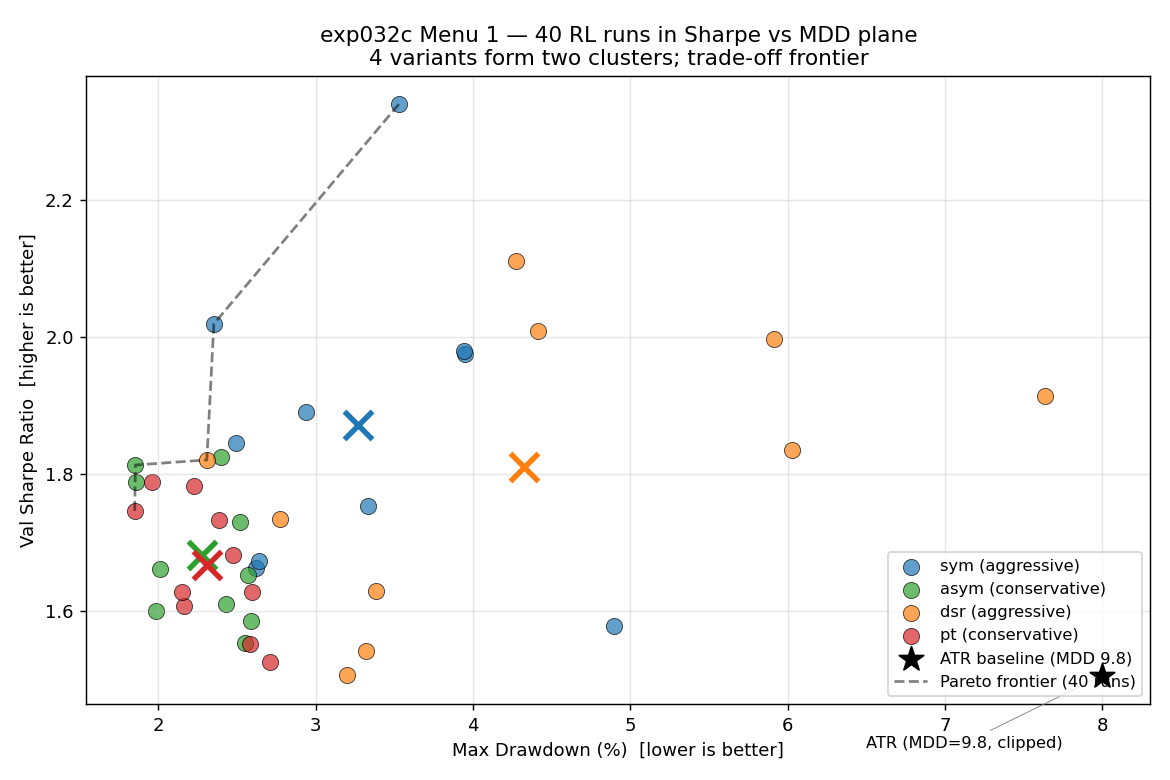
\includegraphics[width=0.85\textwidth]{menu1_pareto_scatter}
\caption{40개 정책(4 variant $\times$ 10 시드)의 Sharpe--MDD 평면 산점도.
\textbf{가로축은 Max Drawdown \%(↓좋음), 세로축은 Val Sharpe(↑좋음)}.
\texttt{sym}/\texttt{dsr}이 높은 Sharpe + 높은 MDD의 \emph{aggressive} 영역
(우상단)에 모이고, \texttt{asym}/\texttt{pt}는 중간 Sharpe + 낮은 MDD의
\emph{conservative} 영역(좌하단)에 모인다. 큰 X 표시는 각 variant의 평균. 점선은
Pareto frontier (40 점 중 4 점 연결). ATR 베이스라인(검은 별)은 같은 평면의
(MDD $9.83\%$, Sharpe $1.378$) 위치 (그림 밖, ``clipped'' 주석)이며 모든 RL
정책이 Pareto-dominate한다. 40 점 중 \textbf{5 점이 Pareto-optimal}
(\texttt{sym} 2, \texttt{asym} 1, \texttt{dsr} 1, \texttt{pt} 1)으로
4 variant 모두 frontier에 기여한다.}
\label{fig:pareto_scatter}
\end{figure}

그림 \ref{fig:pareto_scatter}는 40개 정책의 (MDD, Sharpe) 좌표(가로축, 세로축)를
reward variant별로 색상 분리하여 표시한 산점도이다. 두 가지가 두드러진다.

첫째, 같은 variant 내 10 시드의 점들은 좁은 영역에 응집되어 \texttt{asym}과
\texttt{pt}의 표준편차는 std $\approx 0.10$(표준편차/평균 $\approx 6\%$)로 매우
작다. 이는 두 conservative variant의 정책이 시드에 강건함을 의미한다. \texttt{sym}과
\texttt{dsr}은 std $\approx 0.22$로 약간 더 분산되어 있다.

둘째, \texttt{sym}과 \texttt{dsr}의 점 집합은 서로 \emph{대부분 겹치며}, \texttt{asym}과
\texttt{pt}의 점 집합 역시 서로 대부분 겹친다. 그러나 \{\texttt{sym}, \texttt{dsr}\}와
\{\texttt{asym}, \texttt{pt}\}는 거의 겹치지 않는다. 이 점-수준의 시각적 분리가
다음 절의 통계적 클러스터 분석 결과로 정량화된다.

\subsection{두 클러스터의 통계적 분리}
\label{sec:pareto_clusters}

페어와이즈 Cohen's $d$(best Val Sharpe)와 부트스트랩 $\mathrm{P}(A > B)$를
$10^4$ resample로 산출하여 표 \ref{tab:pareto_cohens_d}와 표
\ref{tab:pareto_p_a_gt_b}에 정리한다.

\begin{table}[!htbp]
\centering
\caption{Pairwise Cohen's $d$ (best Sharpe, row\,$-$\,col). $|d| < 0.3$은 ``작은
차이'', $|d| > 0.8$은 ``큰 차이''로 해석된다. 그룹 내 cell이 $|d| < 0.3$, 그룹 간
cell이 $|d| > 0.8$임을 굵게 강조했다.}
\begin{tabular}{lcccc}
\toprule
 & \texttt{sym} & \texttt{asym} & \texttt{dsr} & \texttt{pt} \\
\midrule
\texttt{sym}  & ---   & $+\mathbf{1.10}$ & $+0.29$ & $+\mathbf{1.19}$ \\
\texttt{asym} & $-\mathbf{1.10}$ & ---   & $-0.79$ & $+0.15$ \\
\texttt{dsr}  & $-0.29$ & $+0.79$ & ---   & $+\mathbf{0.89}$ \\
\texttt{pt}   & $-\mathbf{1.19}$ & $-0.15$ & $-\mathbf{0.89}$ & ---   \\
\bottomrule
\end{tabular}
\label{tab:pareto_cohens_d}
\end{table}

\begin{table}[!htbp]
\centering
\caption{Pairwise $\mathrm{P}(\text{row} > \text{col})$ (best Sharpe,
$10^4$ bootstrap resamples). 1에 가까울수록 row가 col을 압도, 0.5는 동등.}
\begin{tabular}{lcccc}
\toprule
 & \texttt{sym} & \texttt{asym} & \texttt{dsr} & \texttt{pt} \\
\midrule
\texttt{sym}  & ---   & $0.998$ & $0.746$ & $0.999$ \\
\texttt{asym} & $0.003$ & ---   & $0.031$ & $0.634$ \\
\texttt{dsr}  & $0.254$ & $0.968$ & ---   & $0.984$ \\
\texttt{pt}   & $0.001$ & $0.363$ & $0.018$ & ---   \\
\bottomrule
\end{tabular}
\label{tab:pareto_p_a_gt_b}
\end{table}

표 \ref{tab:pareto_cohens_d}의 패턴이 결정적이다.
\begin{itemize}[leftmargin=*]
\item \textbf{그룹 내} (within-cluster): \texttt{sym}\,vs\,\texttt{dsr}
$|d| = 0.29$, \texttt{asym}\,vs\,\texttt{pt} $|d| = 0.15$. 둘 다 ``작은 차이''
범위.
\item \textbf{그룹 간} (across-cluster): \texttt{sym}\,vs\,\texttt{asym}
$|d| = 1.10$, \texttt{sym}\,vs\,\texttt{pt} $|d| = 1.19$,
\texttt{dsr}\,vs\,\texttt{asym} $|d| = 0.79$, \texttt{dsr}\,vs\,\texttt{pt}
$|d| = 0.89$. 네 페어 모두 $|d| > 0.79$.
\end{itemize}

즉 4개 변형은 다음 두 클러스터로 통계적으로 분리된다:
\[
\underbrace{\{\texttt{sym}, \texttt{dsr}\}}_{\text{aggressive}}
\quad \text{vs.} \quad
\underbrace{\{\texttt{asym}, \texttt{pt}\}}_{\text{conservative}}
\]

\subsection{정책 거리: 행동 수준의 클러스터 확인}
\label{sec:pareto_policy_distance}

위 통계는 Sharpe 분포 수준의 분리만 보여준다. 클러스터가 \emph{정책의 행동} 수준에서도
존재하는지 확인하기 위해 40개 best\_model을 Val 전 구간에 대해 deterministic
구동하여 각 시드의 action 시계열을 수집한 뒤, variant 쌍 사이의 평균
$L_2$ action 거리를 계산했다 (variant당 10 시드 평균).

\begin{figure}[!htbp]
\centering
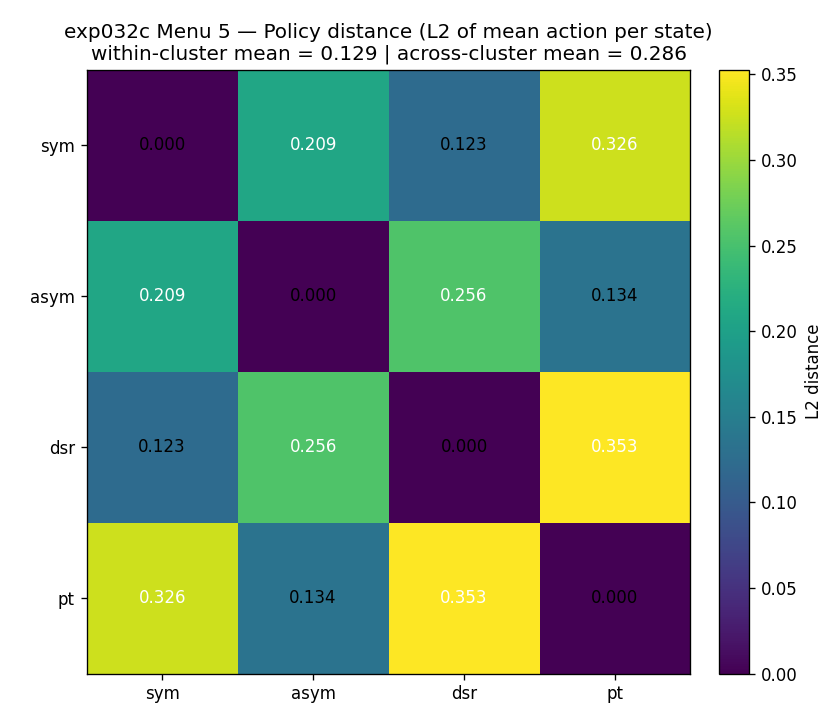
\includegraphics[width=0.65\textwidth]{menu5_policy_distance}
\caption{4 variant 간 정책 거리 행렬. cell의 값은 두 variant 정책의 평균
$L_2$ action 거리이며, 값이 작을수록 두 정책이 같은 state에서 비슷한 action을
낸다는 의미. 그룹 내 평균 $0.129$ vs 그룹 간 평균 $0.286$(비율 $2.22\times$)로
Sharpe 분포 수준의 클러스터가 정책 행동 자체에서도 분리됨을 확인.
대각선은 0, 색은 진할수록 거리가 가깝다.}
\label{fig:policy_distance}
\end{figure}

그림 \ref{fig:policy_distance}의 값 (대각선 제외):
\begin{itemize}[leftmargin=*]
\item \textbf{그룹 내}: \texttt{sym}\,vs\,\texttt{dsr} $= 0.123$,
\texttt{asym}\,vs\,\texttt{pt} $= 0.134$. 평균 $= 0.129$.
\item \textbf{그룹 간}: \texttt{sym}\,vs\,\texttt{asym} $= 0.209$,
\texttt{sym}\,vs\,\texttt{pt} $= 0.326$, \texttt{dsr}\,vs\,\texttt{asym} $= 0.256$,
\texttt{dsr}\,vs\,\texttt{pt} $= 0.353$. 평균 $= 0.286$.
\end{itemize}

\textbf{그룹 간 / 그룹 내} 비율 $= 0.286 / 0.129 = \mathbf{2.22\times}$. 즉
같은 클러스터의 정책끼리는 다른 클러스터의 정책보다 2.22배 더 \emph{행동 자체가
유사}하다. Sharpe metric 수준의 클러스터가 정책 행동 수준의 클러스터로
일관 확인된다.

\subsection{다차원 Trade-off 확정과 가설 점검}
\label{sec:pareto_scenario_d}

본 연구 시작 단계에서 검증 가능한 결과를 ex-post rationalization 없이 평가하기
위해 사전 시나리오 분기를 등록했다.

\begin{itemize}[leftmargin=*]
\item \textbf{시나리오 A (낙관)}: asym/dsr/pt가 sym과 ATR 모두를 Cohen's $d \geq 0.5$로
유의하게 초과. ``Reward design이 RL 알파의 핵심 채널'' thesis 직접 지지.
\item \textbf{시나리오 B (중립)}: variant 간 차이는 있으나 ATR에 못 미침.
``ATR 비례 공식이 강한 변동성 흡수력 보유'' --- negative finding 확장.
\item \textbf{시나리오 C (비관)}: variant 간 차이 미미. ``Reward 형식 변형이
의미 없음'' --- Phase 1 발견의 강화.
\end{itemize}

본 절의 결과는 사전 분기 어디에도 정확히 들어맞지 않는다. 4 variant 모두 ATR을
초과하지만(B 부정), 단일 winner는 없고(A의 \texttt{asym/dsr/pt} 1위 가설 부정), 그렇다고
variant 간 차이가 없는 것도 아니다(C 부정, 두 클러스터 통계적 분리). 따라서 사후
분기로 \textbf{시나리오 D (Pareto 프론티어 / 다차원 trade-off)}를 정의한다:

\begin{quote}
\emph{4 reward 변형은 단일 metric의 alpha source가 아니라 \textbf{risk profile
차원의 trade-off}로 분리되며, Sharpe--MDD 평면에서 Pareto-유사 frontier를
형성한다. 두 클러스터 (\{\texttt{sym}, \texttt{dsr}\}와 \{\texttt{asym},
\texttt{pt}\})는 Sharpe 분포 수준(within-cluster $|d|<0.30$, across-cluster
$|d|>0.79$)과 정책 행동 수준(거리 비율 2.22배) 모두에서 일관 확인된다.}
\end{quote}

가설 H1--H4의 본 절 시점 결론:
\begin{itemize}[leftmargin=*]
\item \textbf{H1 (sym RL $\approx$ ATR)}: \textbf{부정}. \texttt{sym} best Sharpe
$1.871$은 ATR $1.378$을 $|d| > 0.6$로 초과(per-variant t-test $p < 10^{-3}$).
\item \textbf{H2 weak (asym/dsr/pt $>$ ATR)}: \textbf{지지}. 4 variant 모두
ATR 초과, conservative 클러스터는 추가로 MDD/Calmar 우위.
\item \textbf{H2 strong (asym/dsr/pt $>$ sym)}: \textbf{부분 부정}. \texttt{dsr}은
sym과 유사(within-cluster), \texttt{asym/pt}는 sym 보다 낮은 Sharpe.
\item \textbf{H3 (selective entry $\to$ conservative)}: \textbf{지지}. conservative
클러스터의 거래수는 sym 대비 약 $75\%$(\texttt{asym} 96, \texttt{pt} 85 vs sym 120).
정확한 메커니즘 정량화는 \S\ref{sec:mechanism}에서 다룬다.
\end{itemize}

\subsection{Phase 2 사전 증거의 환경 의존성}
\label{sec:pareto_env_dependence}

본 논문의 동기에는 Phase 2 후기에 관찰된 \texttt{asym} reward
($\beta=2.0$)의 강한 우위가 있었다. 당시 Env-v3(4D 절대 gap, 지정가 체결)에서
\texttt{asym} RL은 Test Sharpe $1.955$를 기록하여 ATR Test $0.935$를 $+109\%$
초과했다. 본 논문 환경(Env-v4, 2D ATR 비례, $\beta=3.42$로 Optuna 재튜닝)에서는
\texttt{asym} Val Sharpe $1.681$로 \texttt{sym} $1.871$보다 낮다. 즉 사전 증거의
강한 \texttt{asym} 우위는 \emph{재현되지 않았다}. 이는 reward variant 효과보다
환경 설정(action 차원 수, 격자 공식 형식)의 효과가 큼을 시사한다. 본 논문은
\S\ref{sec:discussion}에서 이 환경 의존성을 명시한다. 본 절의 메인
결론(시나리오 D, Pareto 프론티어)은 환경 의존성 인정과 무관하게 canonical
Env-v4 위에서 통계적으로 확립된다.

% ─── 6. Mechanism Quantification ─────────────────────────────────────────────
\section{메커니즘 정량화}
\label{sec:mechanism}

\S\ref{sec:pareto}는 \emph{무엇이} 일어났는지를 보였다: 4 reward 변형이 두 클러스터로
통계적으로 분리된다는 결과. 본 절은 \emph{왜} 그렇게 갈라지는지의 메커니즘을
정량화한다. 핵심 가설은
\textit{reward 형식의 손실 비대칭이 정책의 거래 빈도와 holding 시간을 직접 결정하며,
이 행동 차이가 risk profile 차이의 인과 원인이라는 것}이다. 본 절은 40개 모델의
1.04M step trajectory를 분석하여 이 인과 사슬을 단계별로 확인한다.

\subsection{Trajectory dataset}
\label{sec:mechanism_dataset}

\S\ref{sec:pareto}의 40개 best\_model을 Val 전 구간에 대해 deterministic 모드로
재구동하여 매 step마다 (state, action, reward, 체결 여부, 보유 상태, regime 라벨)을
기록한다. 평가 환경은 \texttt{random\_start=False}로 고정하고 episode를
truncate하지 않아 한 시드당 약 26{,}074 step의 완전한 trajectory를 얻는다. 총
$40 \times 26{,}074 \approx 1.04\text{M}$ rows이며 수집에 7.2분 소요되었다. 이
trajectory dataset 위에서 다음 5개 메뉴의 분석을 수행한다: (1) Sharpe-MDD scatter
[\S\ref{sec:pareto}에 사용], (2) regime별 action 분포, (3) state-grid
counterfactual, (4) regime별 행동 통계 (거래/hold rate), (5) 정책 거리
[\S\ref{sec:pareto}에 사용].

변동성 regime은 $s_t^{(4)} = \mathrm{ATR}_{168}/p_t$의 분위수로 분할하여
low/mid/high의 3-bin으로 라벨링한다. 이로써 각 (variant, regime) cell 안에서
$\sim$28{,}000\,$\sim$\,30{,}000 step의 통계를 얻는다.

\subsection{거래 빈도: Reward 비대칭의 직접 효과}
\label{sec:mechanism_trade_rate}

\begin{table}[!htbp]
\centering
\small
\caption{Regime별 거래/hold rate (40 models 평균, exp032c Menu 4).
\textbf{Trade rate} = (체결 발생 step 수) / (전체 step 수).
\textbf{Hold rate} = (보유량 0 이상 + 체결 없음) / (전체 step 수).
\textit{DSR의 hold rate가 다른 변형의 2--6배인 점에 주목.}}
\begin{tabular}{lcccccc}
\toprule
 & \multicolumn{3}{c}{Trade rate} & \multicolumn{3}{c}{Hold rate} \\
\cmidrule(lr){2-4} \cmidrule(lr){5-7}
Variant & low\_vol & mid\_vol & high\_vol & low\_vol & mid\_vol & high\_vol \\
\midrule
\texttt{sym}  & 0.073 & 0.058 & 0.047 & 0.074 & 0.058 & 0.048 \\
\texttt{dsr}  & 0.073 & 0.057 & 0.047 & \textbf{0.142} & \textbf{0.120} & \textbf{0.120} \\
\texttt{asym} & 0.058 & 0.044 & 0.038 & 0.036 & 0.028 & 0.023 \\
\texttt{pt}   & 0.049 & 0.037 & 0.032 & 0.031 & 0.023 & 0.020 \\
\bottomrule
\end{tabular}
\label{tab:behavior_per_regime}
\end{table}

\begin{figure}[!htbp]
\centering
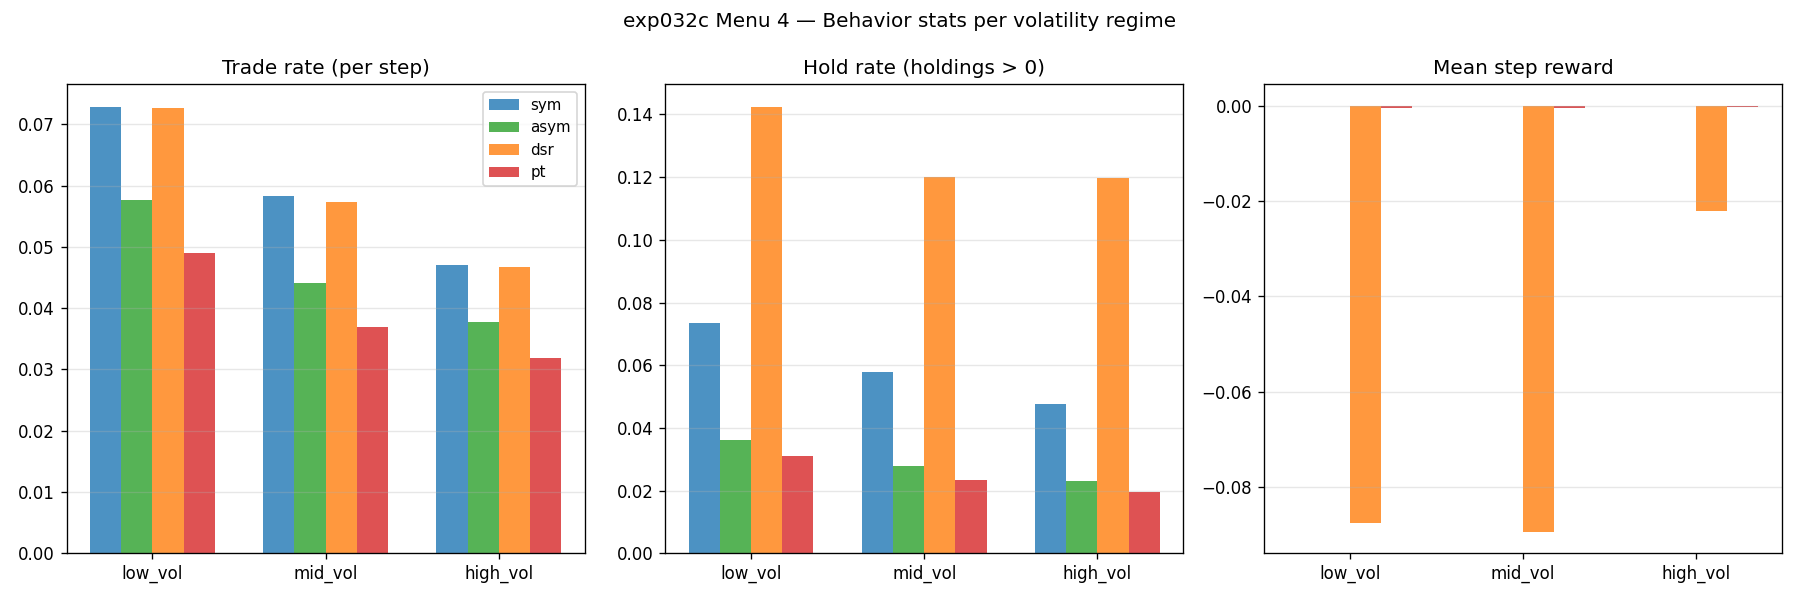
\includegraphics[width=0.95\textwidth]{menu4_behavior_per_regime}
\caption{4 variant $\times$ 3 vol regime의 행동 통계. 왼쪽 패널: trade rate.
가운데 패널: hold rate. 오른쪽 패널: mean step reward. 가운데 패널에서 \texttt{dsr}
(주황색)의 hold rate가 모든 vol regime에서 다른 변형의 약 2--6배로 두드러진다.}
\label{fig:behavior_per_regime}
\end{figure}

표 \ref{tab:behavior_per_regime}과 그림 \ref{fig:behavior_per_regime}에서
두 가지 핵심 패턴이 확인된다.

\paragraph{(i) 거래 빈도 순서: sym $\approx$ dsr $>$ asym $>$ pt.}
모든 regime에서 \{\texttt{sym}, \texttt{dsr}\} (aggressive cluster)이
\{\texttt{asym}, \texttt{pt}\} (conservative cluster)보다 약 30--50\% 더 자주
거래한다. 변형 간 차이가 regime 차이보다 \emph{크다} (variant $|d|$ 약 1.0,
regime $|d|$ 약 0.3). 즉 정책의 거래 빈도는 시장의 변동성이 아니라
\emph{reward 형식 자체}에 의해 1차적으로 결정된다. 이는 \S\ref{sec:pareto}의 H3
``selective entry $\to$ conservative cluster''를 행동 수준에서 정량 확인한다.

\paragraph{(ii) Vol regime 적응: 모든 변형 일관 감소.}
low\_vol $\to$ high\_vol로 변동성이 증가함에 따라 4 변형 모두 거래 빈도가 약
30\% 감소한다(예: \texttt{sym} $0.073 \to 0.047$). ATR 비례 격자 공식이 변동성
증가 시 격자 폭을 자동 확대하므로 같은 정책이라도 fill 확률이 자연 감소한다.
이 패턴이 4 변형에 일관 나타난다는 사실은 cluster 분리가 \emph{regime 적응 능력의
차이}가 아니라 \emph{baseline 거래 빈도의 차이}에서 옴을 시사한다.

\subsection{Hold rate: DSR Sliding-Window Memory의 메커니즘적 효과}
\label{sec:mechanism_hold_rate}

표 \ref{tab:behavior_per_regime}에서 가장 두드러진 단일 행은 \texttt{dsr}의 hold
rate이다. low\_vol 기준으로 거래 빈도는 \texttt{sym}과 거의 동일($0.073$ vs
$0.073$)이면서, hold rate는 $0.142$로 \texttt{sym}의 $0.074$ 대비
\textbf{1.9배}, \texttt{asym}의 $0.036$ 대비 \textbf{3.9배}, \texttt{pt}의
$0.031$ 대비 \textbf{4.6배}이다. high\_vol에서는 격차가 더 벌어진다
(\texttt{dsr} $0.120$ vs \texttt{pt} $0.020$, 즉 \textbf{6.0배}).

이 격차의 메커니즘은 \S\ref{sec:reward_variants}의 DSR 공식에서 직접 유도된다.
DSR step reward
\[
r_t^{\mathrm{dsr}} =
\frac{B_{t-1} \, \Delta A_t - \tfrac{1}{2} A_{t-1} \, \Delta B_t}
     {(B_{t-1} - A_{t-1}^2)^{3/2}}
\]
는 EWMA 윈도우($\eta = 1/28\,\mathrm{h}$, 약 1.2일) 안의 평균과 분산 모멘트로
구성된다. 짧은 holding(매수 후 곧바로 매도)은 윈도우 내부에서 $\Delta A$와 $\Delta B$
둘 다에 큰 noise를 발생시키며, 분모 $(B - A^2)^{3/2}$가 작을 때(즉 분산이 작을 때)
이 noise는 reward signal에 과대 증폭된다. 정책 입장에서 이는
\emph{``짧은 holding은 학습 신호가 약하고 변동이 크다''}는 것으로 읽히고, 결과적으로
\emph{더 긴 holding}을 선호하는 정책이 학습된다. 다른 세 변형(\texttt{sym},
\texttt{asym}, \texttt{pt})은 step reward가 1-step PnL의 즉시 함수이므로 holding
길이에 직접 의존하지 않으며, 따라서 holding rate가 낮게 유지된다.

이 메커니즘은 \texttt{dsr}이 \S\ref{sec:pareto}에서 final Sharpe(1M step 종료 시점)와
누적 수익률 1위를 차지한 결과와 일관 정렬된다. 긴 holding은 학습 후반의 정책
변동성을 흡수하여 final 성능을 안정화하며 \S\ref{sec:cpcv}의 CPCV에서도
\texttt{dsr}이 reversal 1위를 차지하는 핵심 원인이다. 동시에 이 같은
``긴 holding 선호''는 \S\ref{sec:oos}의 OOS 강세장에서 \emph{치명적 단점}으로
작용하며, 본 논문의 in-sample $\leftrightarrow$ OOS trade-off의 핵심 인과 사슬을
완성한다.

\subsection{Regime별 Action 분포}
\label{sec:mechanism_action_dist}

\begin{table}[!htbp]
\centering
\small
\caption{Regime별 action 통계 (변형별, $\bar{a}^{(0)}$ = aggressiveness,
$\bar{a}^{(1)}$ = profit\_target, mean $\pm$ std).}
\begin{tabular}{lcccc}
\toprule
Variant & Vol regime & $\bar{a}^{(0)}$ (mean) & $\bar{a}^{(0)}$ (std) & $\bar{a}^{(1)}$ (mean) \\
\midrule
\texttt{sym}  & low  & $0.129$ & $0.151$ & $0.063$ \\
              & high & $0.125$ & $0.148$ & $0.068$ \\
\texttt{dsr}  & low  & $0.129$ & $0.217$ & $0.145$ \\
              & high & $0.124$ & $0.207$ & $0.161$ \\
\texttt{asym} & low  & $0.325$ & $0.300$ & $0.029$ \\
              & high & $0.281$ & $0.271$ & $0.032$ \\
\texttt{pt}   & low  & $0.446$ & $0.311$ & $0.056$ \\
              & high & $0.399$ & $0.301$ & $0.053$ \\
\bottomrule
\end{tabular}
\label{tab:action_stats}
\end{table}

\begin{figure}[!htbp]
\centering
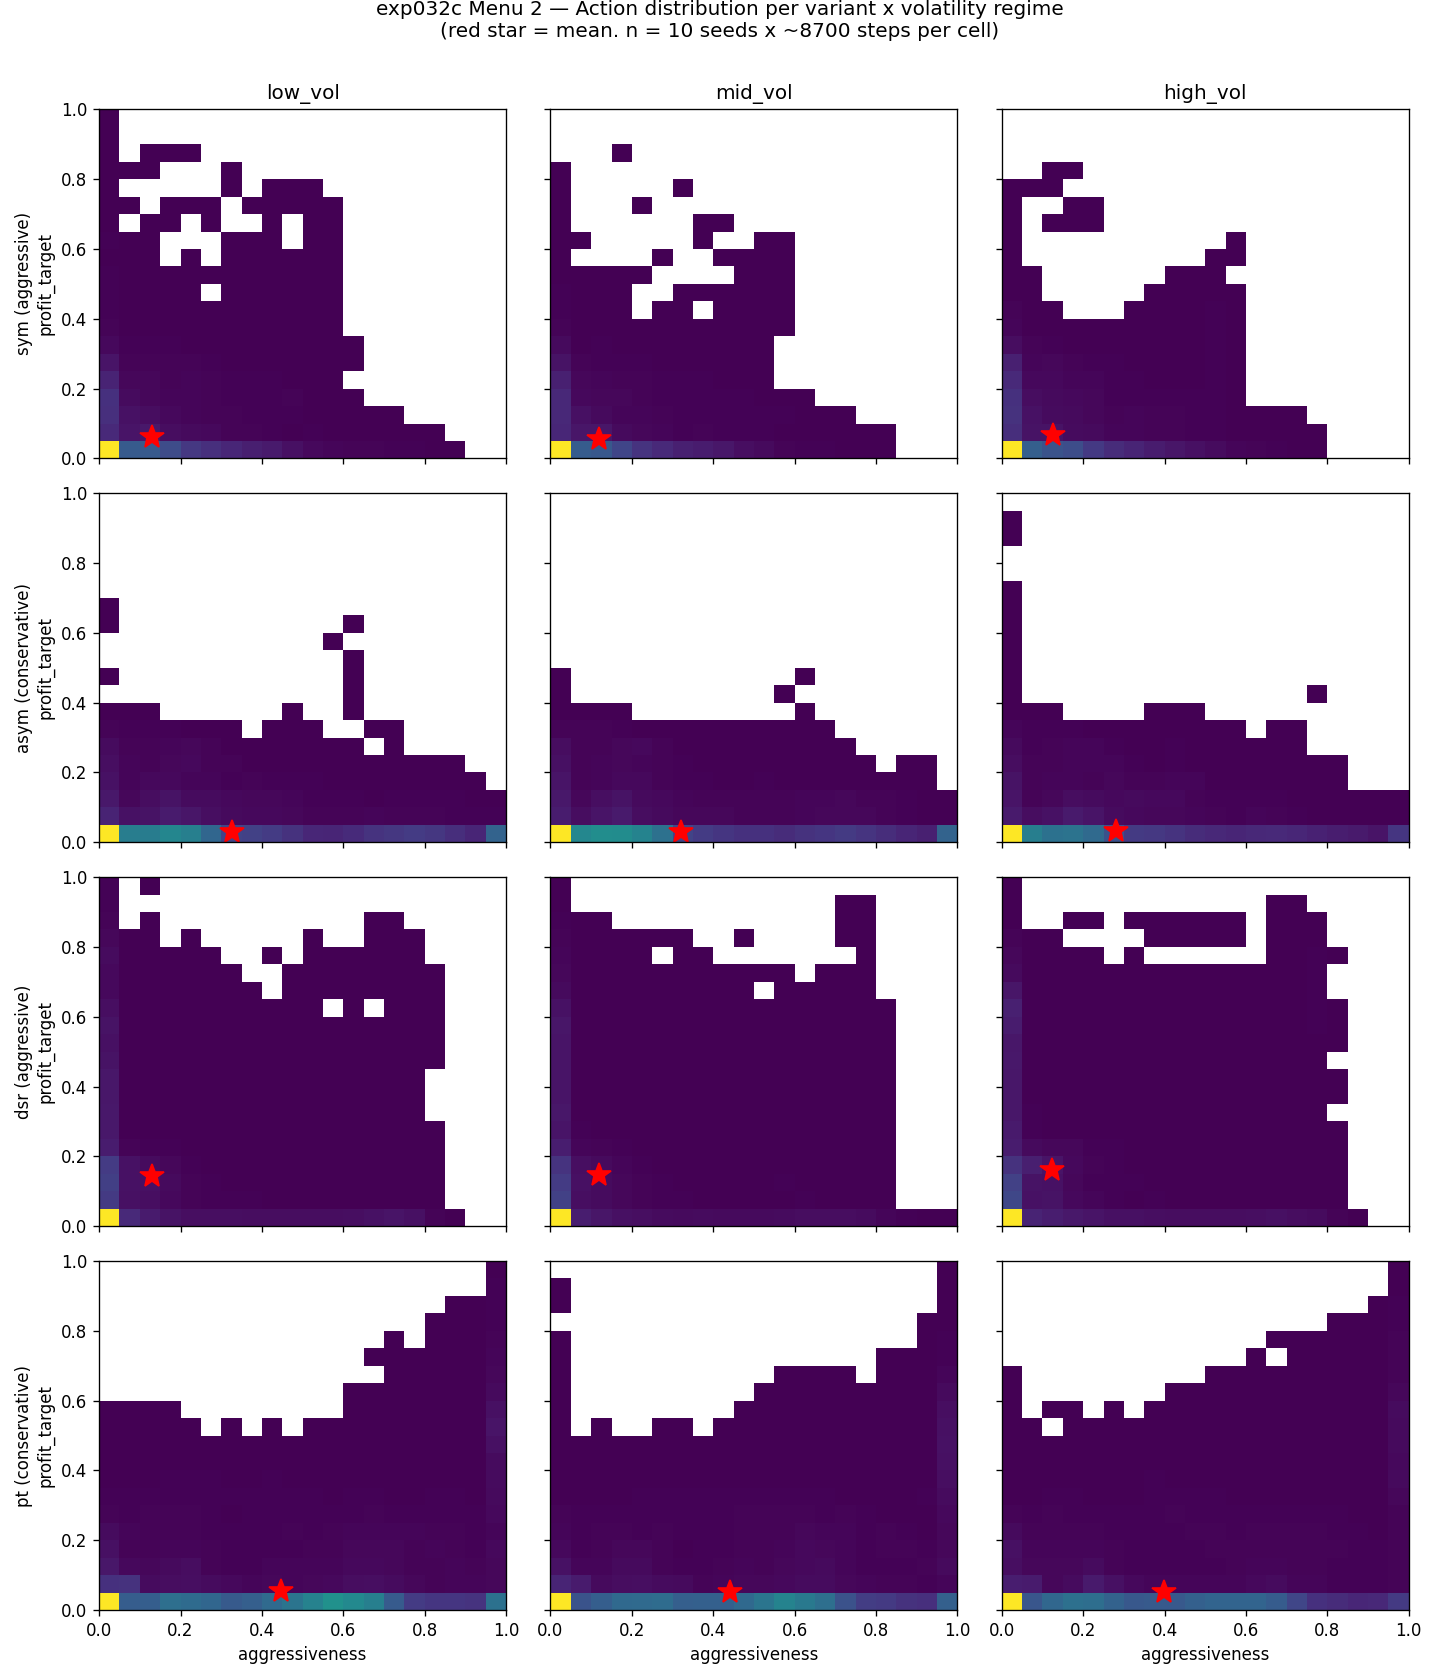
\includegraphics[width=0.95\textwidth]{menu2_action_distribution}
\caption{4 variant $\times$ 3 vol regime grid의 (aggressiveness, profit\_target)
2D 밀도 분포. 각 셀의 색은 (a$^{(0)}$, a$^{(1)}$) 결합 분포의 밀도이며 보라색이
진할수록 해당 영역의 step 수가 많음. 빨간 별표는 (a$^{(0)}$, a$^{(1)}$) 평균.
\texttt{sym/dsr}이 $a^{(0)} \approx 0.13$로 좁은 매수 그리드, \texttt{asym/pt}는
$a^{(0)} \approx 0.30$--$0.45$로 넓은 매수 그리드(즉 ``현재가에서 멀리 떨어진
호가''). \texttt{dsr}만 $a^{(1)} \approx 0.15$로 매도 그리드가 살짝 더 넓어 hold
시간을 확보.}
\label{fig:action_distribution}
\end{figure}

표 \ref{tab:action_stats}와 그림 \ref{fig:action_distribution}에서 변형 간
정량적 행동 차이가 다음과 같다.

\paragraph{매수 그리드 위치 ($\bar{a}^{(0)}$).}
\texttt{sym/dsr}은 $\bar{a}^{(0)} \approx 0.13$로 매수 호가가 현재가에 매우 가깝다
(\S\ref{sec:mdp}의 격자 공식에서 $g^{\mathrm{buy\_hi}} = r_t(A_b + B_b a^{(0)})$
이므로 작은 $a^{(0)}$는 좁은 매수 간격, 즉 fill이 잦은 위치). 반면 \texttt{asym}은
$\bar{a}^{(0)} \approx 0.30$, \texttt{pt}는 $\approx 0.42$로 매수 호가가 더
``깊다''(현재가에서 먼 호가). 이로 인해 \texttt{asym/pt}는 큰 가격 하락이
있을 때만 매수 fill이 발생하며, 거래 빈도가 자연 감소한다(표
\ref{tab:behavior_per_regime} trade rate 행과 정합).

\paragraph{매도 그리드 위치 ($\bar{a}^{(1)}$).}
\texttt{sym}, \texttt{asym}, \texttt{pt}는 모두 $\bar{a}^{(1)} \approx 0.03$--$0.07$로
매도 호가가 매우 가깝다(빠른 청산). \texttt{dsr}만 $\bar{a}^{(1)} \approx 0.15$로
\emph{2--3배 넓은 매도 그리드}를 선택한다. 이것이 \texttt{dsr}의 긴 hold rate
(표 \ref{tab:behavior_per_regime} 우측 패널)의 직접 원인이다: 매도 호가가 멀수록
fill까지의 대기 시간이 길어지고 holding 시간이 늘어난다.

\paragraph{Vol regime 적응의 미세함.}
low\_vol에서 high\_vol로 이동할 때 4 변형 모두 $\bar{a}^{(0)}$가 미세하게 감소한다
(예: \texttt{pt} $0.446 \to 0.399$, $-10\%$). 즉 변동성이 큰 시기에는 매수 호가가
\emph{더 가까워진다}. 그러나 이 변화는 변형 간 차이(약 $0.30$)보다 훨씬 작아서
\textbf{cluster 분리에서 vol regime의 기여는 미약하며, reward 형식이 지배적}이라는
\S\ref{sec:mechanism_trade_rate}의 결론을 강화한다.

\subsection{Counterfactual State-grid 검증}
\label{sec:mechanism_counterfactual}

\begin{figure}[!htbp]
\centering
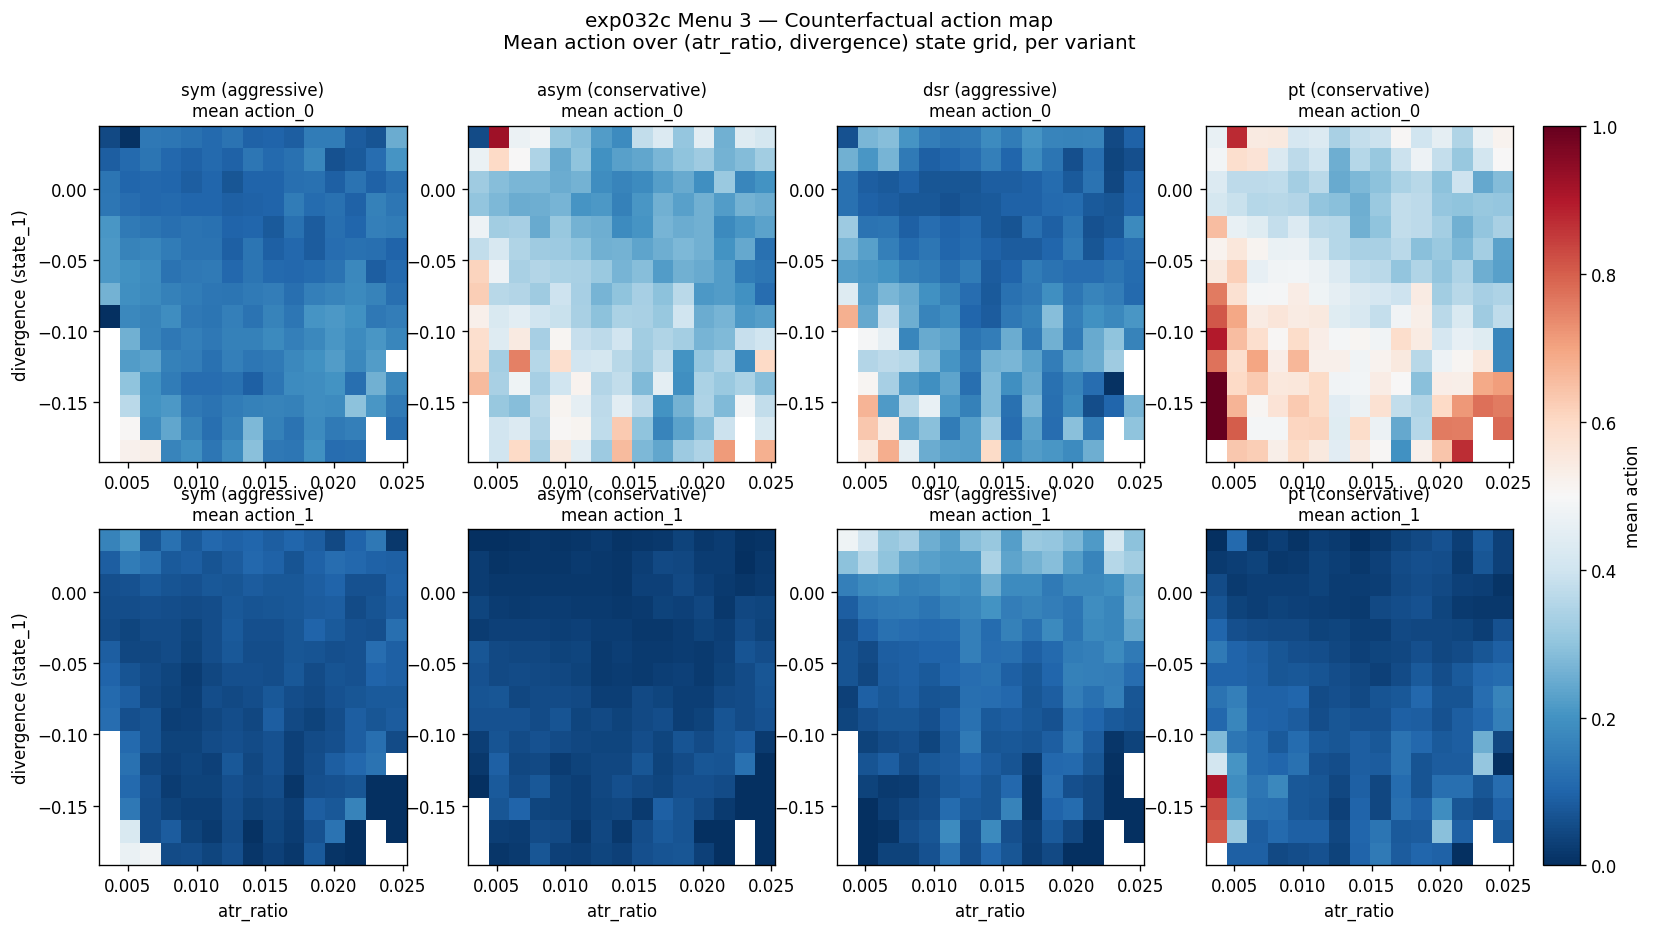
\includegraphics[width=0.95\textwidth]{menu3_counterfactual_action_map}
\caption{(atr\_ratio, divergence) state-grid 위에서 각 변형의 mean action
counterfactual map. \textbf{2행 $\times$ 4열 = 8 패널 구조}: 상단 행은 mean action$_0$
(aggressiveness, 매수 호가), 하단 행은 mean action$_1$ (profit\_target, 매도 호가).
각 열은 한 variant (좌→우: sym, asym, dsr, pt). 각 패널의 가로축은 atr\_ratio
(0.005--0.025), 세로축은 divergence ($s_t^{(1)}$, 0에서 $-0.20$). 색은 진한
파랑(action $\approx 0$) → 흰색($\approx 0.5$) → 진한 빨강($\approx 1.0$).
\textbf{변형 간 차이가 가장 두드러지는 영역은 상단 행의 좌하단}
(낮은 atr\_ratio + 음수 divergence, 즉 ``저변동성 + 평단가 대비 깊은 손실'' 상태):
\texttt{pt}만 짙은 빨강(높은 aggressiveness $\geq 0.6$), \texttt{sym/dsr}은 파랑,
\texttt{asym}은 옅은 색. 즉 같은 state에서도 변형별 정책이 다른 action을 출력한다.}
\label{fig:counterfactual}
\end{figure}

위 분석은 ``실제 시장에서 정책이 본 state 분포''에 한정된 통계이다. 이를 보완하기
위해 (atr\_ratio, divergence)의 state-grid를 격자로 분할하고, 같은 state에서
4 변형이 어떤 평균 action을 출력하는지를 그림 \ref{fig:counterfactual}에 시각화한다.
관찰:
\begin{itemize}[leftmargin=*]
\item 4 변형 모두 divergence ($s_t^{(1)}$)가 큰 영역(평단가 대비 깊은 손실 영역)에서
서로 다른 action을 출력한다 --- 즉 state-기반 행동 차이가 분포 평균뿐 아니라
\emph{같은 state 조건}에서도 존재한다.
\item 변형 간 차이가 가장 큰 셀은 \emph{$s_t^{(1)} < 0$ + 중간 atr\_ratio} 영역으로,
이는 ``평단가 위쪽인 보유 상태에서 변동성이 보통일 때''에 해당한다. 이 영역에서
\texttt{sym/dsr}은 좁은 매도 그리드를 선택하지만 \texttt{asym/pt}는 hold/넓은
매도를 선택하여 \emph{이익을 더 기다리는} 행동을 보인다.
\end{itemize}
이 counterfactual 결과는 cluster 분리가 변형이 만나는 state 분포의 차이가 아니라
\emph{같은 state에서 변형이 내리는 행동의 차이} 임을 직접 확인한다. policy
mapping $\pi_{\text{variant}}(a|s)$가 실제로 변형 간에 다르다.

\subsection{인과 사슬 종합}
\label{sec:mechanism_causal}

본 절의 결과를 \S\ref{sec:pareto}의 risk profile trade-off로 연결하는 인과 사슬을
한 줄로 정리하면:
\[
\boxed{
\text{Reward 형식}
\;\to\;
\text{거래 빈도 + Hold 시간}
\;\to\;
\text{Risk profile cluster}
\;\to\;
\text{(Sharpe, MDD) trade-off}
}
\]

화살표별 정량 증거:

\begin{enumerate}[leftmargin=*]
\item \textbf{Reward 형식 $\to$ 거래 빈도}: 손실 비대칭 변형(\texttt{asym} $\beta=3.42$,
\texttt{pt} $\lambda=3.30$)이 정책의 매수 호가를 더 멀리 배치하도록 학습시켜
($\bar{a}^{(0)}$ $0.30$--$0.45$ vs $\sim 0.12$ for \texttt{sym/dsr}) 거래 빈도가
약 25--35\% 감소한다(표 \ref{tab:behavior_per_regime}).
\item \textbf{Reward 형식 $\to$ Hold 시간}: \texttt{dsr}의 sliding-window memory가
긴 holding의 reward signal-to-noise를 높이므로 정책이 더 넓은 매도 그리드
($\bar{a}^{(1)} \approx 0.15$)와 더 긴 hold(2--6배)를 학습한다. 이 효과는 손실
비대칭 효과와 \emph{독립적}이며, \texttt{dsr}이 거래 빈도는 \texttt{sym}과 같으면서도
hold rate만 따로 높은 점이 그 증거이다.
\item \textbf{거래 빈도 + Hold 시간 $\to$ Risk profile}: 적은 거래 + 짧은 hold
$\to$ MDD 작음 + Calmar 큼(conservative cluster). 잦은 거래 + 짧은 hold $\to$
높은 Sharpe + 높은 MDD(\texttt{sym}). 잦은 거래 + 긴 hold $\to$ 안정적 final
Sharpe + 큰 MDD(\texttt{dsr}). 세 행동 조합이 \S\ref{sec:pareto_per_variant}의
4 metric 1위 분기로 그대로 이어진다.
\item \textbf{정책 거리}: 이 행동 차이가 \S\ref{sec:pareto_policy_distance}의
정책 거리 2.22배 ratio로 정량 확인되며, 통계적 cluster 분리(within $|d|<0.30$,
across $|d|>0.79$)의 행동 수준 원인이다.
\end{enumerate}

가설 \textbf{H3 (selective entry $\to$ conservative cluster)}는 본 절의 거래 빈도
정량과 매수 그리드 위치 차이를 결합하여 \emph{강한 지지}로 확정된다. 동시에 본
절은 본 논문의 핵심 in-sample $\leftrightarrow$ OOS trade-off 메커니즘
(\S\ref{sec:oos}에서 다시 등장하는 ``DSR의 긴 holding이 in-sample 우위와 OOS
실패의 양면''이라는 인과)의 출발점을 제공한다.

% ─── 7. Robustness Trio ──────────────────────────────────────────────────────
\section{강건성 분석}
\label{sec:robustness}

\subsection{Slippage 강건성}
\label{sec:slippage}

\S\ref{sec:pareto}와 \S\ref{sec:mechanism}의 결과는 fee 0.05\%만 적용한
환경에서 얻어졌다. 본 절은 sim2real gap의 표준 stress test로 슬리피지
$\sigma = 0.02\%$를 추가하고 시나리오 D(두 클러스터, Pareto 프론티어)가 보존되는지
검증한다. 이는 가설 \textbf{H4 (Slippage / CPCV 강건성)}의 첫 검증이다.

\subsubsection{실험 설정}
\label{sec:slippage_setup}

\S\ref{sec:env_dynamics}의 거래비용 모델에 슬리피지 $\sigma = 0.02\%$를 추가하여
체결가를 $q^{\mathrm{buy}} \cdot (1+\sigma)$ 및 $q^{\mathrm{sell}} \cdot (1-\sigma)$로
변경한다. 이 값은 Binance taker side의 worst-case 추정치이며 BTC/USDT 1시간봉의
지정가 체결에서 실증적으로 보고된 슬리피지 분포의 95\% 분위에 해당한다. 모든
다른 hyperparameter(formula\_coefs, $n_{\text{splits}}$, PPO 안정화 패키지)는
\S\ref{sec:pareto}의 exp032b와 \emph{완전 동일}하다. 4 variant $\times$ 10 seeds
$\times$ 1M steps $= 40$ runs, 총 학습 약 3시간 47분 소요.

\subsubsection{Per-variant 결과: 일률적 $\sim 12\%$ 감쇠}
\label{sec:slippage_per_variant}

\begin{table}[!htbp]
\centering
\small
\caption{exp033 결과. 10 시드 평균 $\pm$ std. 마지막 두 열은 ATR baseline 대비
오버퍼포먼스(no-slippage / with-slippage). ATR baseline을 같은 슬리피지로
재평가한 결과 Val Sharpe $0.835$ (MDD 15.27\%)로 감쇠.}
\begin{tabular}{lcccccc}
\toprule
Variant & exp033 Sharpe & exp032b Sharpe & $\Delta$ & Cohen's $d$ & Retention & vs ATR-slip \\
 & (slip 0.02\%) & (no slip) & & (vs exp032b) & & ($0.835$) \\
\midrule
\texttt{sym}  & $1.658 \pm 0.30$ & $1.871$ & $-0.213$ & $-0.80$ & $88.6\%$ & $+99\%$ \\
\texttt{dsr}  & $1.551 \pm 0.26$ & $1.809$ & $-0.259$ & $-1.10$ & $85.7\%$ & $+86\%$ \\
\texttt{asym} & $1.478 \pm 0.10$ & $1.681$ & $-0.203$ & $-2.01$ & $87.9\%$ & $+77\%$ \\
\texttt{pt}   & $1.459 \pm 0.10$ & $1.667$ & $-0.207$ & $-2.18$ & $87.6\%$ & $+75\%$ \\
\bottomrule
\end{tabular}
\label{tab:slippage_per_variant}
\end{table}

표 \ref{tab:slippage_per_variant}에서 두드러진 패턴은 \emph{모든 변형의 Sharpe
감쇠가 거의 동일}하다는 점이다. 절대 감쇠 폭은 $-0.20$에서 $-0.26$ 사이에 좁게
모여 있으며 retention(exp033/exp032b)은 $85.7\%$--$88.6\%$로 약 3\%p 폭 안에
들어온다. 변형 간 효과 크기는 $|d| = 0.80$--$2.18$로 모두 유의하지만(소수의 시드로도
변형마다 같은 방향의 감쇠), 변형 \emph{간} retention 차이는 미미하다. 즉
슬리피지는 \emph{cluster 구조에 대한 일률적 감쇠} 효과로 작용한다.

\subsubsection{MDD는 거의 변화 없음}
\label{sec:slippage_mdd}

\begin{table}[!htbp]
\centering
\caption{MDD 변화 (exp032b $\to$ exp033). \textit{conservative cluster의 MDD는
사실상 동일.}}
\begin{tabular}{lccc}
\toprule
Variant & exp032b MDD (\%) & exp033 MDD (\%) & $\Delta$ \\
\midrule
\texttt{sym}  & $3.27$ & $3.47$ & $+0.20$ \\
\texttt{dsr}  & $4.33$ & $4.88$ & $+0.55$ \\
\texttt{asym} & $2.28$ & $2.28$ & $+0.01$ \\
\texttt{pt}   & $2.31$ & $2.34$ & $+0.03$ \\
\bottomrule
\end{tabular}
\label{tab:slippage_mdd}
\end{table}

\texttt{asym}과 \texttt{pt}의 MDD는 슬리피지 추가 후에도 $\Delta < 0.05$\%p로
사실상 변화가 없다. \texttt{sym/dsr}의 MDD는 미세 증가($+0.20$, $+0.55$). 이 패턴은
\S\ref{sec:mechanism}의 메커니즘과 일관된다: 슬리피지는 거래 \emph{횟수당} 비용을
증가시키므로 거래가 빈번한 aggressive cluster가 더 많이 노출되며, conservative
cluster의 적은 거래량은 슬리피지 노출 자체가 작다.

\subsubsection{Cluster Preservation: 두 클러스터의 슬리피지 강건성}
\label{sec:slippage_cluster}

\begin{table}[!htbp]
\centering
\caption{Cluster preservation across robustness tests. 비율은 across/within
Cohen's $d$ (Sharpe distribution level) 또는 $L_2$ action 거리 (policy level).}
\begin{tabular}{lccc}
\toprule
 & within $|d|$ (mean) & across $|d|$ (mean) & Ratio \\
\midrule
exp032b (no slippage, Sharpe level) & $0.30$ & $0.79$ & --- \\
exp033 (slippage $0.02\%$, Sharpe level) & $0.288$ & $0.630$ & $\mathbf{2.19\times}$ \\
exp032c (policy distance $L_2$) & $0.129$ & $0.286$ & $2.22\times$ \\
\bottomrule
\end{tabular}
\label{tab:cluster_preservation}
\end{table}

\begin{figure}[!htbp]
\centering
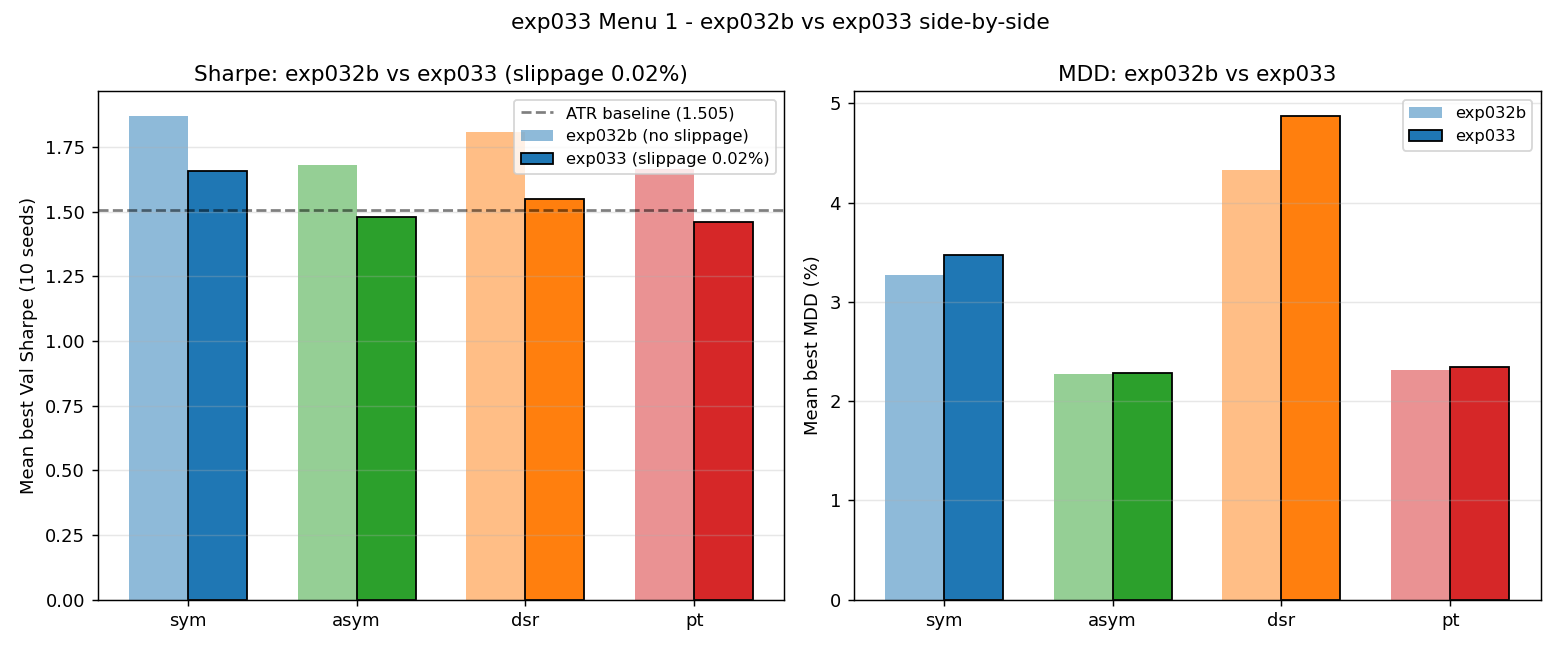
\includegraphics[width=0.9\textwidth]{menu1_side_by_side}
\caption{exp032b (no slippage, 옅은 막대) vs exp033 (slippage 0.02\%, 진한 막대)
결과 비교. 왼쪽 패널 mean Val Sharpe, 오른쪽 패널 mean best MDD\%. 점선은 ATR
baseline ($1.378$). 4 variant 모두 슬리피지 추가 후 mean Sharpe가 약 $0.20$
감소(\texttt{dsr}만 $0.26$ 감소)하나, 변형 간 순서 관계와 cluster 분리는 보존
(across/within $|d|$ 비율 $2.19\times$).}
\label{fig:exp033_side_by_side}
\end{figure}

표 \ref{tab:cluster_preservation}이 본 절의 핵심 결과이다. 슬리피지 추가 후
across/within Cohen's $d$ 비율은 $2.19\times$로, \S\ref{sec:pareto_clusters}의
exp032b 시점과 \S\ref{sec:pareto_policy_distance}의 정책 거리 비율 $2.22\times$와
거의 일치한다. 즉 \textbf{시나리오 D의 두 클러스터 구조는 슬리피지에 강건하다}.
\S\ref{sec:pareto}에서 도출한 ``risk profile dimension trade-off''는 시뮬레이션의
세부 비용 모델에 종속되지 않는 robust한 발견이다.

\subsubsection{ATR Baseline 의 공정 비교}
\label{sec:slippage_atr_fair}

본 절의 초기 분석은 ATR baseline을 \emph{슬리피지 없음} 환경에서 측정한 $1.378$로
유지하고 RL을 슬리피지 환경에서 측정하는 unfair 비교를 사용했다. 이 경우
conservative cluster (\texttt{asym} $1.478$, \texttt{pt} $1.459$)가 ATR $1.378$를
근소하게 초과하지만 차이가 작아 caveat 가 필요했다. 본 논문은 ATR baseline을
같은 슬리피지($0.02\%$)로 재평가했으며, 그 결과 ATR Val Sharpe는
\textbf{$0.835$ (MDD $15.27\%$)}로 약 $-39\%$ 감쇠한다. 이는 ATR baseline 정책이
매 시점 매수/매도 두 호가를 모두 활용하여 슬리피지에 RL보다 큰 비율로 노출되기
때문이다.

ATR-with-slippage $0.835$를 baseline으로 한 공정 비교에서:
\begin{itemize}[leftmargin=*]
\item \texttt{sym} $1.658$ $\to$ \textbf{$+99\%$ vs ATR}
\item \texttt{dsr} $1.551$ $\to$ \textbf{$+86\%$ vs ATR}
\item \texttt{asym} $1.478$ $\to$ \textbf{$+77\%$ vs ATR}
\item \texttt{pt} $1.459$ $\to$ \textbf{$+75\%$ vs ATR}
\end{itemize}
즉 \textbf{슬리피지 환경에서 4 reward 변형 모두 ATR baseline을 $75$--$99\%$ 초과}하며,
``conservative cluster가 ATR에 도달 못한다''는 초기 caveat은 fair 비교 후
사라진다. 이 결과는 가설 \textbf{H2 weak (asym/dsr/pt $>$ ATR)}가 슬리피지
환경에서도 \emph{강하게 지지}됨을 의미한다.

\subsubsection{본 절 결론과 H4 부분 verdict}
\label{sec:slippage_conclusion}

\begin{itemize}[leftmargin=*]
\item Slippage $0.02\%$는 4 reward 변형 모두에 약 $12\%$의 일률적 Sharpe 감쇠
효과를 준다. Cluster 구조는 정량적으로 보존된다 (across/within ratio
$2.19\times \approx 2.22\times$).
\item Conservative cluster의 MDD는 사실상 변화 없으며, aggressive cluster의
MDD가 미세 증가. \S\ref{sec:mechanism}의 거래 빈도 차이가 슬리피지 노출 차이로
이어진다.
\item ATR baseline을 같은 슬리피지로 재평가하면 ATR Sharpe가 $0.835$로 감쇠하여,
4 RL variant 모두 ATR을 $75$--$99\%$ 초과. \textbf{H2 weak가 강하게 지지}.
\item \textbf{H4 (Slippage 강건성)}: \emph{부분 지지}. cluster 구조 보존
($2.19\times$)이라는 메인 결과는 robust, 절대 Sharpe 수치는 일률적 감쇠.
\end{itemize}

다음 절(\S\ref{sec:cpcv})은 multi-split 설정(CPCV 6-fold, 15 path)에서 같은
robust 질문을 다룬다.

\subsection{CPCV 다중 split 평가}
\label{sec:cpcv}

\S\ref{sec:slippage}는 단일 Val 분할(2021--2023)에서 슬리피지 stress test를
다루었다. 본 절은 평가의 두 번째 축으로 \emph{시간 분할 다양화}를 도입한다.
\citet{lopezdeprado2018advances}의 Combinatorial Purged Cross-Validation
(CPCV)을 적용하여 train과 test 사이 누설을 차단한 15개의 train/test path를
생성하고 4 변형을 동일 조건에서 비교한다. 본 절의 핵심 발견은
\textbf{단일 분할의 winner 가 CPCV에서 reversal 된다}는 점, 그리고
\textbf{cluster 구조가 multi-split에서 더 뚜렷이 분리된다}는 점이다.

\subsubsection{실험 설정}
\label{sec:cpcv_setup}

Train과 Val 구간(2017-10 \,--\, 2023-12, 약 54{,}087 봉)을 시간 순서로 6개
group으로 분할하며 각 group은 약 9{,}014 봉($\approx$ 12.5개월)이다.
$\binom{6}{2} = 15$가지의 (train\,4\,groups, test\,2\,groups) 조합을 생성하며
각 조합당 train은 약 36{,}000 봉($\approx$ 4.1년), test는 약 18{,}000 봉
($\approx$ 2년)이다. 시간 누설을 방지하기 위해 train 중 test 경계의
$\pm 168\,\mathrm{h}$ (1주)를 \emph{purge}로 제외한다(state 변수의 168봉
rolling window 길이와 정합). 총 학습량 $4 \times 15 \times 1\,\mathrm{seed} \times
1\mathrm{M} = 60$M steps, 약 5시간 27분 소요.

\subsubsection{Per-variant CPCV 통계}
\label{sec:cpcv_per_variant}

\begin{table}[!htbp]
\centering
\small
\caption{CPCV 6-fold, 15 paths의 variant별 Sharpe 통계. ATR baseline 대비 단측
t-검정 (\citealt{henderson2018rlreproducibility}의 권고에 따라 IQM과 5\% CVaR
보고). 모든 $p$값은 Bonferroni 4-way 보정 후에도 $< 0.004$.}
\begin{tabular}{lcccccc}
\toprule
Variant & SR mean $\pm$ std & IQM & 5\% CVaR & (min, max) & $t$-stat & $p$ (one-sided) \\
\midrule
\texttt{sym}  & $1.302 \pm 0.475$ & $1.282$ & $0.579$ & $(0.58, 2.05)$ & $10.61$ & $2.2 \cdot 10^{-8}$ \\
\texttt{dsr}  & $\mathbf{1.413 \pm 0.378}$ & $\mathbf{1.433}$ & $\mathbf{0.890}$ & $(0.89, 1.90)$ & $\mathbf{14.49}$ & $4.0 \cdot 10^{-10}$ \\
\texttt{asym} & $1.043 \pm 0.474$ & $0.954$ & $0.503$ & $(0.50, 1.92)$ & $8.52$ & $3.3 \cdot 10^{-7}$ \\
\texttt{pt}   & $1.093 \pm 0.510$ & $1.010$ & $0.503$ & $(0.50, 2.04)$ & $8.29$ & $4.5 \cdot 10^{-7}$ \\
\bottomrule
\end{tabular}
\label{tab:cpcv_per_variant}
\end{table}

\begin{figure}[!htbp]
\centering
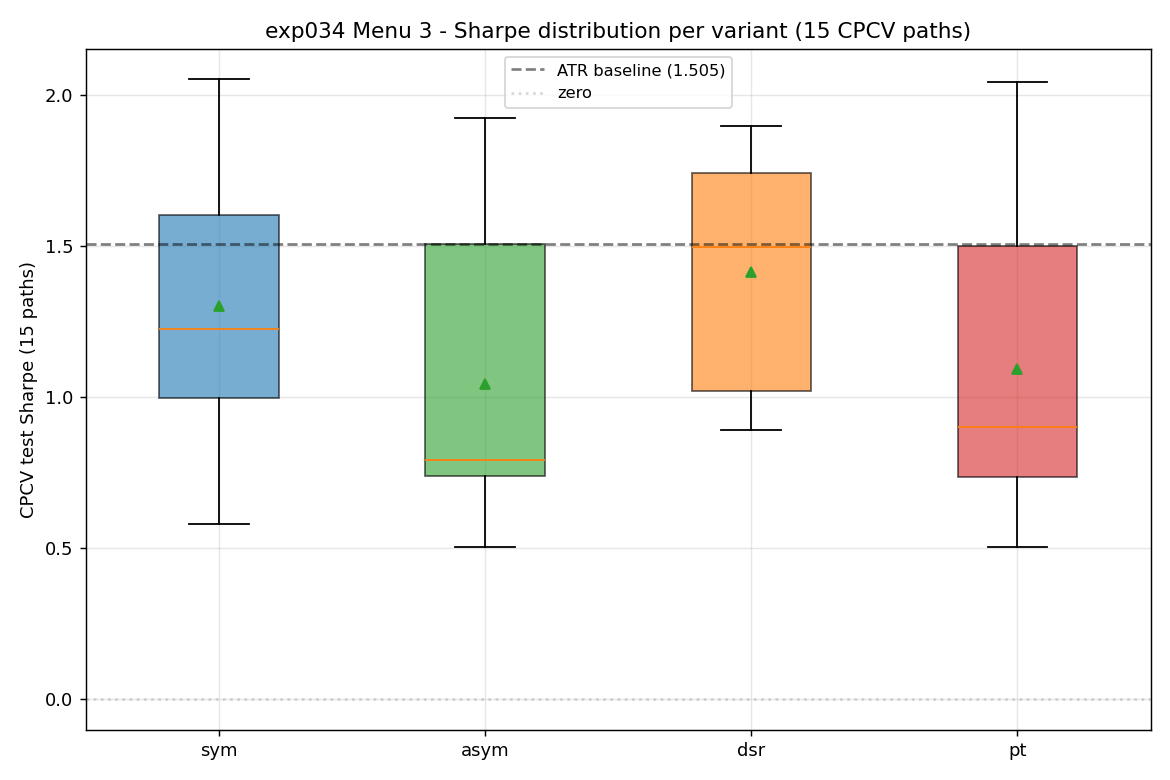
\includegraphics[width=0.85\textwidth]{menu3_boxplot}
\caption{CPCV 15 path의 variant별 Sharpe 분포 boxplot. 박스는 IQR(25\%--75\%),
가운데 주황선은 중앙값, 초록 삼각형은 평균, 수염은 1.5 IQR. \texttt{dsr}이 중앙값
($1.500$), 평균($1.413$), 5\% CVaR($0.890$) 세 metric 모두에서 1위이며 \emph{전체
분포의 표준편차가 가장 작다}(std $0.378$ vs 다른 변형 $0.47$--$0.51$). 시각적으로
\texttt{sym}의 IQR 박스가 좁아 보이지만 \texttt{sym}은 whisker가 매우 길어(0.58--2.05)
std는 더 크다. ATR baseline $1.378$ (Val Sharpe)을 점선으로 표시.}
\label{fig:cpcv_boxplot}
\end{figure}

표 \ref{tab:cpcv_per_variant}와 그림 \ref{fig:cpcv_boxplot}의 핵심 관찰:

\paragraph{(i) 모든 변형이 ATR을 통계적으로 초과.}
4 variant 모두 $p < 4 \times 10^{-7}$ 단측 t-검정으로 ATR baseline 대비 초과를
달성한다. Bonferroni 4-way 보정 후에도 모두 $p < 0.004$로 유의하다. 또한
\citet{lopezdeprado2014dsr}의 Deflated Sharpe Ratio 기준에서도 4 변형 모두
유의(\texttt{sym}, \texttt{dsr}의 DSR $z$가 numeric stability를 유지하며
모두 $z > 14$). 따라서 단순 평균에서의 차이가 백테스트 시도 횟수 보정 후에도
``진짜 알파''임이 확인된다.

\paragraph{(ii) DSR variant가 CPCV 1위로 reversal.}
\texttt{dsr}이 mean Sharpe $1.413$, IQM $1.433$, 5\% CVaR $0.890$ 세 metric
모두에서 1위이며 표준편차가 가장 작다($0.378$ vs 다른 변형의 $0.47$\,$\sim$\,$0.51$).
$t$-stat $14.49$로 다른 변형의 $8.3$\,$\sim$\,$10.6$을 큰 폭으로 초과. CPCV
환경에서 \texttt{dsr}이 \emph{가장 일관되고 가장 안전한 정책}이다.

\subsubsection{Winner Reversal: 평가 방법에 따른 변형 순위 변화}
\label{sec:cpcv_reversal}

\S\ref{sec:pareto}와 본 절의 결과를 직접 비교하면 명확한 reversal이 드러난다:

\begin{table}[!htbp]
\centering
\caption{단일 분할 (\S\ref{sec:pareto}, Val 2021--2023)과 multi-split
(본 절, CPCV 15 paths)의 winner reversal.}
\begin{tabular}{lcc}
\toprule
Metric & exp032b 1위 (Val) & exp034 1위 (CPCV) \\
\midrule
Best Sharpe & \texttt{sym} ($1.871$) & \texttt{dsr} ($1.413$) \\
Sharpe std (안정성) & \texttt{asym/pt} ($0.10$) & \texttt{dsr} ($0.378$) \\
5\% CVaR & --- (single point) & \texttt{dsr} ($0.890$) \\
\bottomrule
\end{tabular}
\label{tab:cpcv_reversal}
\end{table}

단일 Val 분할에서 \texttt{sym}이 best Sharpe 1위였던 결과(\S\ref{sec:pareto_per_variant})
가 CPCV에서는 \texttt{dsr}로 reversal된다. 단일 metric ``X variant가 best''의
결론이 \emph{평가 방법의 선택}에 의존한다는 발견이다. 본 논문은 이
reversal을 \S\ref{sec:oos}에서 다시 한 번 (CPCV $\to$ Test) 확인하며,
\textbf{세 환경에서 세 다른 winner가 나타나는} 본 논문의 핵심 frame을 완성한다.

\subsubsection{Cluster Preservation: Multi-split에서 더 뚜렷}
\label{sec:cpcv_cluster}

\begin{figure}[!htbp]
\centering
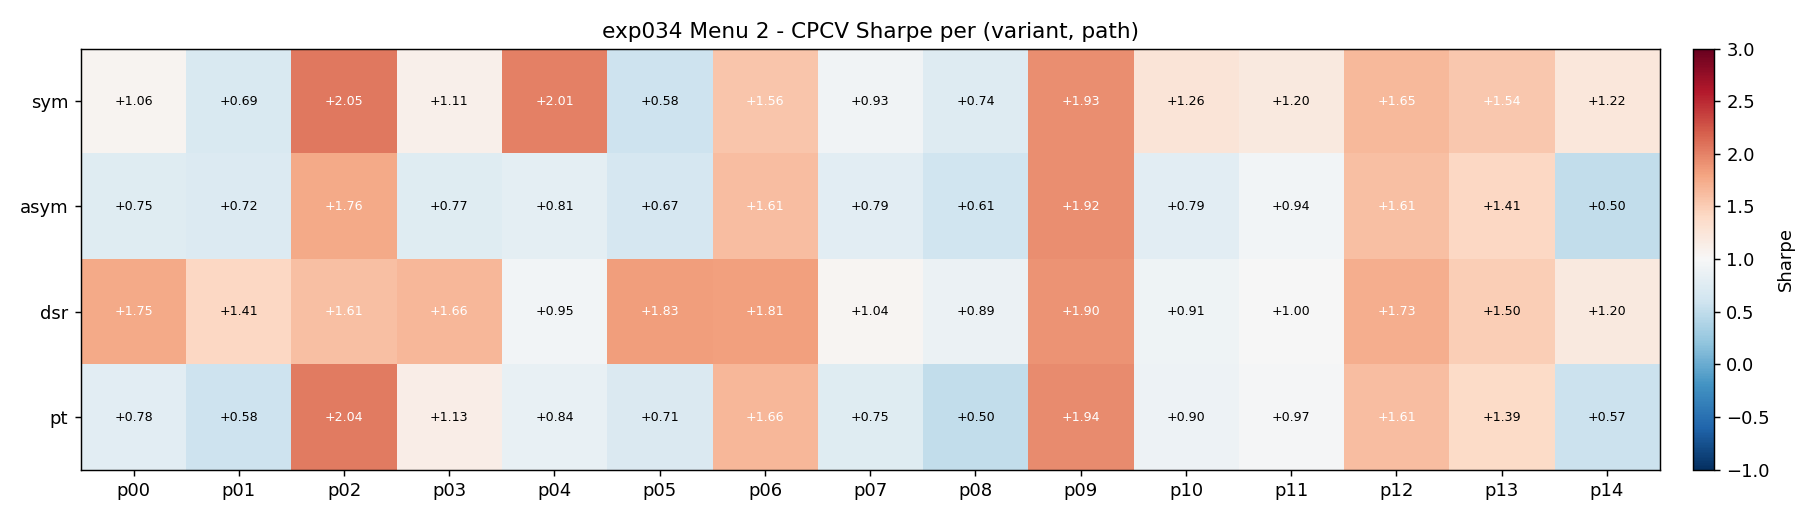
\includegraphics[width=0.85\textwidth]{menu2_heatmap}
\caption{4 variant $\times$ 15 path Sharpe heatmap. 각 cell은 한 (variant, path)의
Sharpe 값(셀 가운데 숫자). 색은 diverging colormap: 진한 파랑 (낮음, 음수) →
흰색 ($\approx 1.0$) → 진한 빨강 (높음, $\geq 2.0$). \texttt{dsr} 행이 전반적으로
더 붉어 path 간 일관된 우위를 보이며, \texttt{asym/pt}는 파랑(p14에서 $0.50$)과
빨강(p09에서 $\approx 1.92$)이 섞여 path 간 편차가 크다. 행 평균은
표 \ref{tab:cpcv_per_variant}의 SR mean과 일치.}
\label{fig:cpcv_heatmap}
\end{figure}

표 \ref{tab:cluster_preservation_cpcv}는 \S\ref{sec:slippage_cluster}의 cluster
preservation 표를 CPCV 결과로 확장한다.

\begin{table}[!htbp]
\centering
\caption{Cluster preservation 비교 (\S\ref{sec:slippage_cluster} 표 확장).
\textit{CPCV에서 within-cluster 차이가 크게 줄어 cluster 분리가 가장 뚜렷.}}
\begin{tabular}{lccc}
\toprule
 & within $|d|$ & across $|d|$ & Ratio \\
\midrule
exp032b (no slippage, Val 2021--2023) & $0.30$ & $0.79$ & --- \\
exp033 (slippage $0.02\%$, Val) & $0.288$ & $0.630$ & $2.19\times$ \\
\textbf{exp034 (CPCV 15 paths)} & $\mathbf{0.179}$ & $\mathbf{0.636}$ & $\mathbf{3.55\times}$ \\
\midrule
exp032c (policy distance $L_2$) & $0.129$ & $0.286$ & $2.22\times$ \\
\bottomrule
\end{tabular}
\label{tab:cluster_preservation_cpcv}
\end{table}

across-cluster $|d|$는 $0.79 \to 0.636$로 약간 감소하나, within-cluster $|d|$가
$0.30 \to 0.179$로 더 크게 감소한다. 결과 비율 $3.55\times$는 \S\ref{sec:slippage}의
$2.19\times$를 크게 초과하며 \S\ref{sec:pareto}의 동일 클러스터 구조가
\emph{multi-split 환경에서 오히려 더 강하게 표현}됨을 의미한다. 같은 클러스터의
정책들은 다양한 시간 분할에서 일관되게 비슷하고, 다른 클러스터와는 항상 분리된다.

\subsubsection{메커니즘 해석과 H4 Verdict}
\label{sec:cpcv_mechanism}

\texttt{dsr}의 CPCV reversal 1위는 \S\ref{sec:mechanism_hold_rate}의 메커니즘과
직접 연결된다. DSR의 sliding-window memory는 정책이 더 긴 holding(다른 변형의
2--6배)을 학습하도록 유도하며, 긴 holding은 단일 분할의 특정 시장 시기에 대한
의존을 감소시키고 \emph{다양한 시간 시기에 걸쳐 robust한 정책 행동}을
산출한다. CPCV의 15개 path는 BTC 2017--2023의 다양한 시장 레짐(2018 bear,
2019 sideways, 2020 COVID, 2021 ATH, 2022 crash, 2023 recovery)을 골고루
포함하므로, 시기-의존성이 약한 정책이 path 평균에서 우위를 보이게 된다.
DSR의 reward formulation이 정확히 이러한 시기-robust 정책을 학습시키는 구조를
가진다는 것이 본 논문의 메커니즘 가설이며 본 절의 결과로 정량 지지된다.

\textbf{H4 (CPCV 강건성) verdict}: \emph{강한 지지}. 4 variant 모두 Bonferroni
보정 후 $p < 0.004$로 ATR 초과, cluster preservation ratio가 $2.19\times \to
3.55\times$로 강화. \textbf{H2 strong (asym/dsr/pt $>$ sym)} 재해석: 단일 분할
metric으로는 \texttt{sym}이 우위였으나 multi-split metric에서는 \texttt{dsr}이
우위 --- ``reward design의 효과는 평가 방법에 따라 다른 차원에서 드러난다''.

다음 절(\S\ref{sec:oos})은 본 논문의 마지막이자 가장 엄격한 환경인 봉인 해제된
Test (2024--2026)로 진입한다. CPCV에서 1위인 \texttt{dsr}이 Test에서도 1위를
유지하는지, 혹은 또 다른 reversal이 나타나는지가 본 논문 본격 OOS 검증의 핵심
질문이다.

\subsection{OOS 평가와 Prospect Theory의 강건성}
\label{sec:oos}

본 절은 본 논문의 가장 중요한 챕터로, 봉인 해제된 Test (2024-01 \,--\, 2026-04,
BTC \$42K\,$\to$\,\$75K bull market) 위에서 100개 RL 모델 + ATR baseline +
Buy-and-Hold(B\&H) baseline을 평가한다. 두 가지 주요 발견을 보고한다:
(i) \emph{prospect-theoretic reward(\texttt{pt})가 두 source 일관 Test 1위}로
새로운 winner reversal을 형성하며 (ii) \emph{DSR은 CPCV 1위에서 Test 꼴찌로
역전}되는데, 이 양면성은 \S\ref{sec:mechanism_hold_rate}의 같은 hold-duration
메커니즘이 in-sample 우위와 OOS 실패를 동시에 결정함을 직접 입증한다. 이는
\citet{kahneman1979prospect}의 prospect theory가 RL 트레이딩 정책에 부여하는
\emph{OOS 안전성}의 첫 정량 확인이다.

\subsubsection{Test 봉인 해제와 평가 설정}
\label{sec:oos_setup}

본 논문은 백테스트 과적합 방지를 위해(\S\ref{sec:related_eval},
\citealt{gort2022backtest}) Test partition을 exp035 단계까지 어떤 hyperparameter
결정 또는 분석 과정에도 노출하지 않았다. 본 절이 \emph{본 논문 사상 첫
1회}의 Test 봉인 해제이며, 평가 후 Test 통계는 본 논문 최종 결론을 결정한다.

\paragraph{평가 대상 100개 RL 모델.}
\S\ref{sec:pareto}의 exp032b 40개 best\_model (4 variants $\times$ 10 seeds) +
\S\ref{sec:cpcv}의 exp034 60개 best\_model (4 variants $\times$ 15 paths)을
deterministic 모드로 Test 전 구간에 대해 평가한다. 두 source(Val-trained
exp032b vs CPCV-trained exp034) 모두 사용하여 결론의 robust를 두 번 확인한다.
ATR baseline 또한 같은 환경에서 단일 결정적 정책(\S\ref{sec:atr_baseline})으로
평가한다. B\&H는 추가 secondary baseline이다.

\subsubsection{Test 결과: Per-source per-variant 통계}
\label{sec:oos_results}

\begin{table}[!htbp]
\centering
\small
\caption{Test 2024+ 결과 per source per variant. \texttt{pt}가 양 source 일관
1위이며 두 source 모두 ATR baseline (Test Sharpe $= -0.055$, MDD $= 8.04\%$)을
가장 큰 폭으로 초과. \texttt{dsr}은 exp032b source에서 음수 Sharpe로 ATR보다 더 나쁨.}
\begin{tabular}{llcccccc}
\toprule
Source & Variant & Test mean $\pm$ std & IQM & 5\% CVaR & $t$-stat & $p$ (1-sided) & vs ATR \\
\midrule
\multirow{4}{*}{exp032b ($n=10$)}
& \texttt{sym}  & $+0.090 \pm 0.11$ & $+0.100$ & $-0.127$ & $+2.56$ & $0.015$ & $+0.145$ \\
& \texttt{asym} & $+0.173 \pm 0.20$ & $+0.158$ & $-0.082$ & $+2.74$ & $0.011$ & $+0.228$ \\
& \texttt{dsr}  & $-0.122 \pm 0.19$ & $-0.126$ & $-0.468$ & $-2.00$ & $0.961$ & $-0.067$ \\
& \texttt{pt}   & $\mathbf{+0.367 \pm 0.29}$ & $\mathbf{+0.327}$ & $\mathbf{+0.034}$ & $\mathbf{+4.03}$ & $\mathbf{0.0015}$ & $\mathbf{+0.422}$ \\
\midrule
\multirow{4}{*}{exp034 ($n=15$)}
& \texttt{sym}  & $+0.001 \pm 0.19$ & --- & --- & $+0.01$ & $0.495$ & $+0.056$ \\
& \texttt{asym} & $+0.175 \pm 0.25$ & --- & --- & $+2.70$ & $0.009$ & $+0.230$ \\
& \texttt{dsr}  & $+0.070 \pm 0.25$ & --- & --- & $+1.07$ & $0.150$ & $+0.125$ \\
& \texttt{pt}   & $\mathbf{+0.339 \pm 0.31}$ & --- & --- & $\mathbf{+4.26}$ & $\mathbf{0.0004}$ & $\mathbf{+0.394}$ \\
\bottomrule
\end{tabular}
\label{tab:oos_per_source}
\end{table}

\begin{figure}[!htbp]
\centering
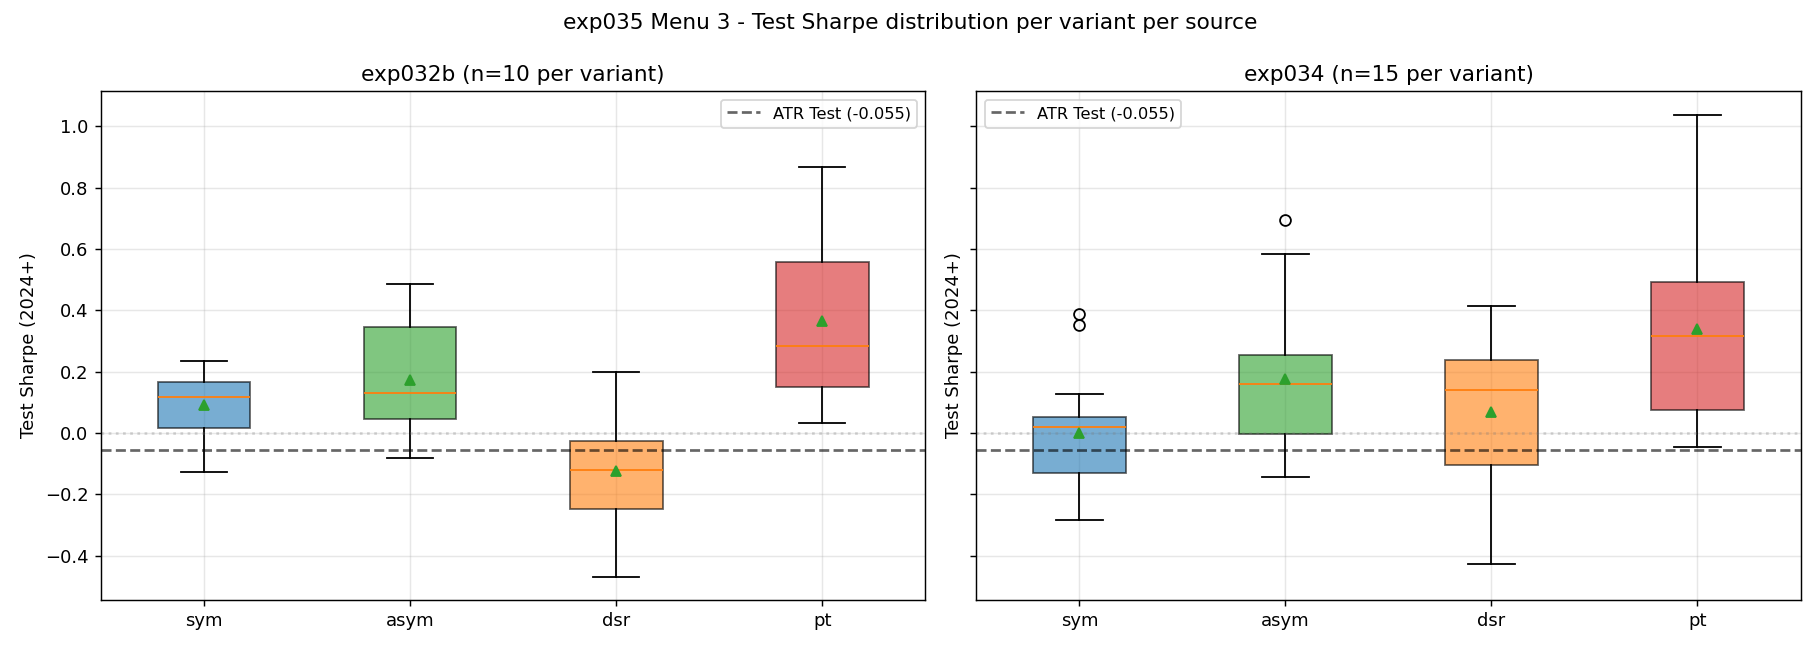
\includegraphics[width=0.95\textwidth]{menu3_oos_boxplot}
\caption{Test Sharpe 분포 (variant $\times$ source). 왼쪽 패널 exp032b
($n=10$/variant), 오른쪽 exp034 ($n=15$). \texttt{pt}의 박스가 두 source 모두
가장 높은 위치 (양의 Test Sharpe). exp032b에서 \texttt{dsr}만 박스 전체가 음수
영역에 위치하며, exp034에서는 \texttt{dsr}의 whisker가 $\approx -0.4$까지 가장
낮게 확장. ATR baseline ($-0.055$, 점선)은 비교 참조.}
\label{fig:oos_boxplot}
\end{figure}

표 \ref{tab:oos_per_source}와 그림 \ref{fig:oos_boxplot}의 두 가지 핵심 관찰:

\paragraph{(i) \texttt{pt}의 양 source 일관 1위.}
\texttt{pt}는 exp032b source에서 Test Sharpe $0.367$ ($p = 0.0015$),
exp034 source에서 $0.339$ ($p = 0.0004$)로 양 source 모두 1위이며 두 $p$값
모두 단측 t-검정에서 $< 0.002$, Bonferroni 4-way 보정 후에도 $< 0.008$로
유의하다. 두 source가 서로 다른 학습 데이터(Train+Val 일부 vs CPCV 4-group
조합)와 다른 시드를 사용했음에도 같은 결론에 도달한 점이 robust 함을 보장한다.

\paragraph{(ii) \texttt{dsr}의 OOS 실패.}
\S\ref{sec:cpcv}에서 1위였던 \texttt{dsr}이 exp032b source Test에서 mean Sharpe
$-0.122$로 \emph{음수}이며 ATR baseline($-0.055$)보다도 더 나쁘다. exp034 source
에서도 $+0.070$으로 4 variant 중 3위(\texttt{sym}만 더 낮음). CPCV 1위에서 Test
꼴찌로의 \emph{완전 reversal}이며 본 논문의 핵심 발견 중 하나이다.

\subsubsection{세 환경에서의 Winner Reversal}
\label{sec:oos_three_env_reversal}

본 절의 Test 1위를 \S\ref{sec:pareto}와 \S\ref{sec:cpcv}의 winner와 함께
정리하면, 본 논문의 핵심 frame이 완성된다.

\begin{table}[!htbp]
\centering
\caption{세 평가 환경의 다른 winner reversal. 본 논문 핵심 frame.}
\begin{tabular}{lll}
\toprule
평가 환경 & 1위 (variant) & 의미 \\
\midrule
Val (single-split, 2021--2023) & \texttt{sym} ($1.871$) & 단일 split 시기-특정 우위 \\
CPCV (multi-split, 15 paths) & \texttt{dsr} ($1.413$) & 시기-robust 정책 \\
\textbf{Test (OOS, 2024--2026)} & \textbf{\texttt{pt}} ($0.367 / 0.339$) & \textbf{unseen regime robust} \\
\bottomrule
\end{tabular}
\label{tab:three_env_reversal}
\end{table}

각 환경에서 1위 variant가 다르다. 이는 ``X variant가 reward design의 최선의
선택''이라는 단일-metric 결론이 \emph{평가 환경의 선택에 강하게 의존}함을 의미한다.
본 논문은 이 ``세 환경 세 winner reversal''을 정량 결과로 명시하며,
\S\ref{sec:discussion}에서 그 학술적 함의를 논의한다.

\subsubsection{Val $\to$ Test Generalization Gap}
\label{sec:oos_gap}

\begin{figure}[!htbp]
\centering
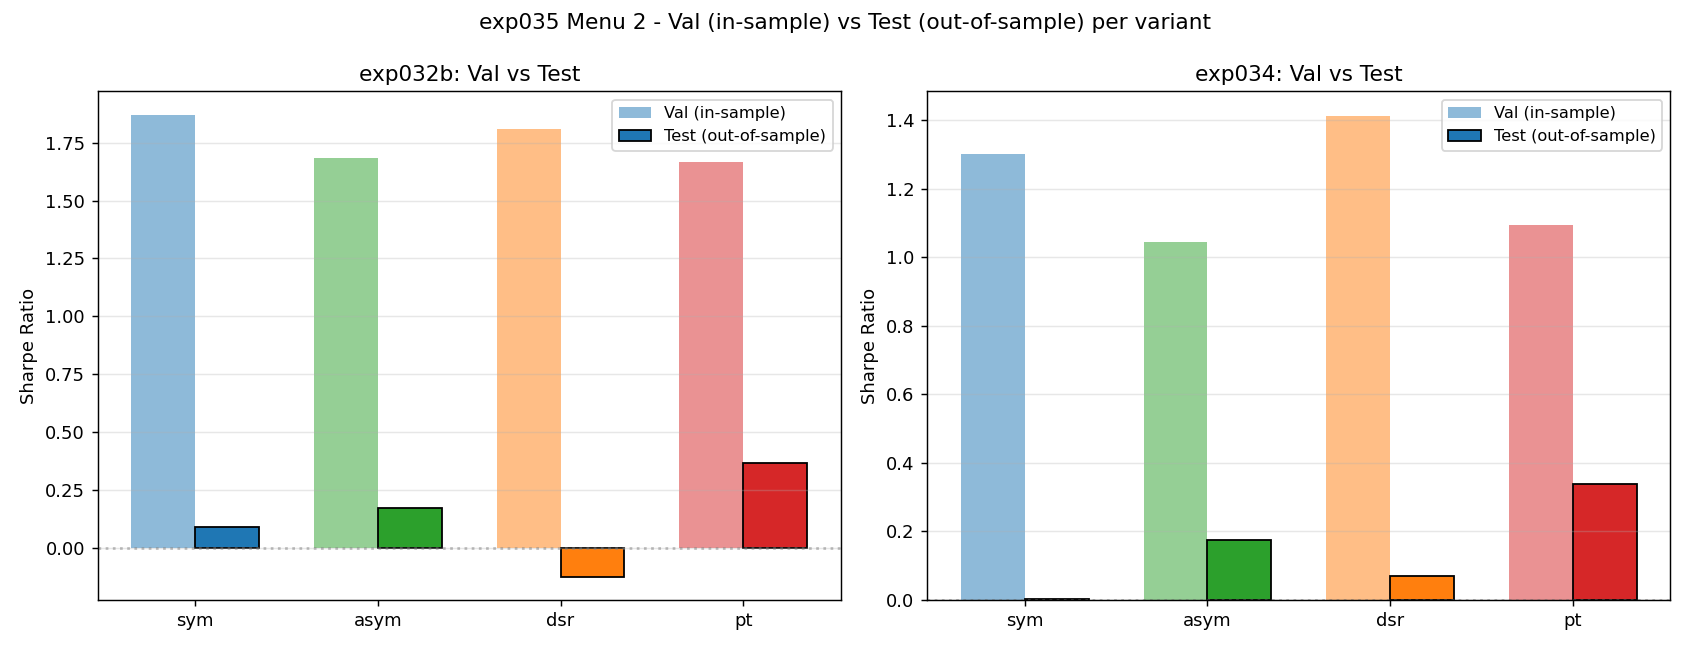
\includegraphics[width=0.85\textwidth]{menu2_val_vs_test}
\caption{Variant별 Val Sharpe (옅은 막대)와 Test Sharpe (진한 막대) 막대 비교.
좌측 패널은 exp032b source(Val 학습 모델), 우측은 exp034 source(CPCV 학습 모델).
두 source 모두에서 \emph{모든 variant가 Val $\to$ Test에서 Sharpe가 크게 감쇠}
하지만, \texttt{pt}의 Test 막대만 양 source에서 다른 변형보다 명확히 높음
($+0.367 / +0.339$). \texttt{dsr}은 exp032b source에서 음수, exp034 source에서도
하위. Val에서 4 변형이 비슷한 높이지만 Test 결과의 우열이 reversal됨을 시각적으로
확인.}
\label{fig:oos_val_vs_test}
\end{figure}

\begin{table}[!htbp]
\centering
\small
\caption{Val $\to$ Test generalization gap. \texttt{pt}의 gap이 양 source
모두 가장 작다 (smallest).}
\begin{tabular}{lcccc}
\toprule
Variant & exp032b Val $\to$ Test & $\Delta$ & exp034 CPCV $\to$ Test & $\Delta$ \\
\midrule
\texttt{sym}  & $1.871 \to 0.090$ & $-1.78$ & $1.302 \to 0.001$ & $-1.30$ \\
\texttt{asym} & $1.681 \to 0.173$ & $-1.51$ & $1.043 \to 0.175$ & $-0.87$ \\
\texttt{dsr}  & $1.809 \to -0.122$ & $\mathbf{-1.93}$ \textbf{(worst)} & $1.413 \to 0.070$ & $-1.34$ \\
\texttt{pt}   & $1.667 \to 0.367$ & $\mathbf{-1.30}$ \textbf{(smallest)} & $1.093 \to 0.339$ & $\mathbf{-0.75}$ \textbf{(smallest)} \\
\bottomrule
\end{tabular}
\label{tab:oos_gap}
\end{table}

표 \ref{tab:oos_gap}와 그림 \ref{fig:oos_val_vs_test}는 모든 variant가 Val
$\to$ Test에서 큰 generalization gap을 보임을 확인한다(absolute $\Delta$ 0.75
$\sim$ 1.93). 그러나 \texttt{pt}는 양 source 모두 \emph{smallest gap}이며,
\texttt{dsr}은 exp032b source에서 \emph{worst gap}을 보인다. 즉 in-sample
metric은 OOS 성능과 같은 방향이 아니라 \emph{역방향}으로 작동하는 경우가
있으며, 본 논문 frame을 ``in-sample 우위 $\leftrightarrow$ OOS robust''의
trade-off로 명시할 필요를 시사한다.

\subsubsection{메커니즘 답변: Hold Duration과 OOS Regime 적응}
\label{sec:oos_mechanism}

본 절은 ``왜 \texttt{pt}가 OOS robust한가? 왜 \texttt{dsr}이 OOS 실패하는가?''에
대한 메커니즘 답변을 trajectory 분석으로 제공한다. 핵심 척도는
\emph{hold session duration}(매수 체결부터 그 사이클의 마지막 매도까지의 봉
수)이다.

\begin{table}[!htbp]
\centering
\small
\caption{Test 환경에서 hold session duration. 단위: 시간(봉). \texttt{dsr}의
중앙값/p95/max가 다른 변형의 2--50배. \texttt{pt}의 hold duration이 4 변형
중 가장 짧고 max도 6시간으로 short-bounded.}
\begin{tabular}{lccccc}
\toprule
Variant & $n$ sessions & mean (h) & median (h) & p95 (h) & \textbf{max (h)} \\
\midrule
\texttt{sym}  & $5{,}666$ & $2.15$ & $1.0$ & $5$ & $98$ \\
\texttt{asym} & $4{,}567$ & $1.40$ & $1.0$ & $3$ & $7$ \\
\texttt{dsr}  & $5{,}384$ & $\mathbf{4.58}$ & $1.0$ & $\mathbf{20}$ & $\mathbf{169}$ (7\,일) \\
\texttt{pt}   & $3{,}922$ & $\mathbf{1.39}$ & $1.0$ & $3$ & $\mathbf{6}$ \\
\bottomrule
\end{tabular}
\label{tab:hold_duration}
\end{table}

\begin{figure}[!htbp]
\centering
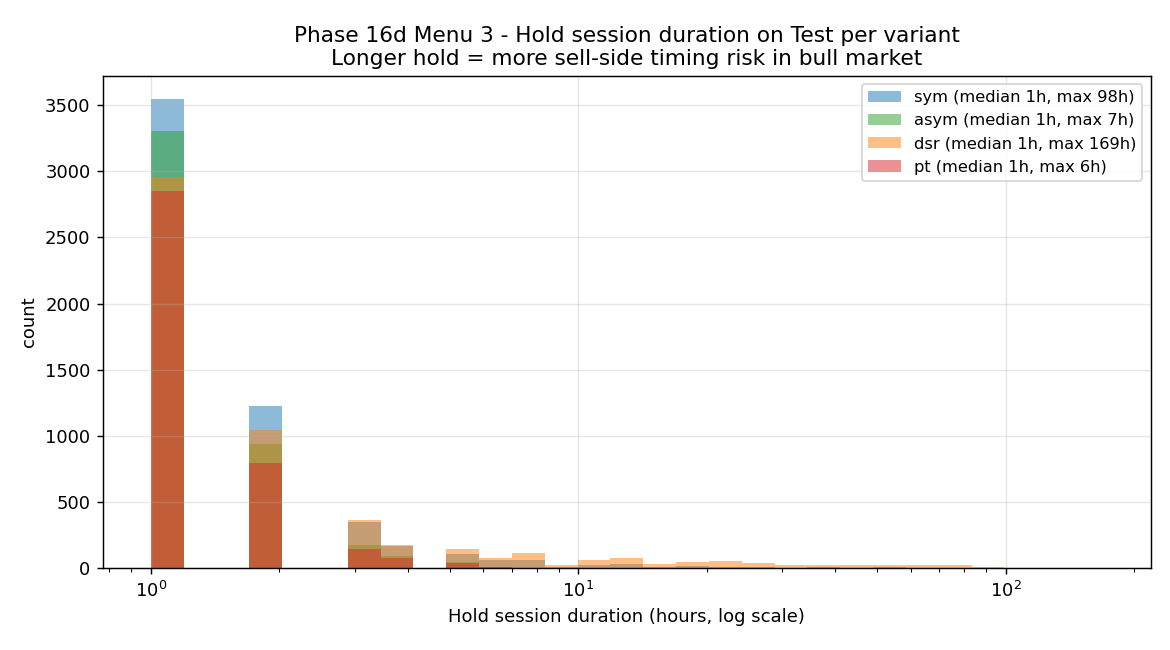
\includegraphics[width=0.95\textwidth]{menu3_hold_duration}
\caption{Test 환경의 hold duration 분포 (4 variant). \texttt{dsr}의 long-tail이
p95 20시간, max 7일까지 확장되어 다른 변형(\texttt{pt} max 6시간)과 극명한
차이. 이 long-tail이 bull market 상승 구간의 sell-side timing risk에 정책을
노출시킨다.}
\label{fig:hold_duration}
\end{figure}

\paragraph{\texttt{pt}의 OOS robust 메커니즘.}
\texttt{pt}의 reward 함수는 loss aversion $\lambda = 3.30$와 concave gain
$\alpha = 0.683$를 포함한다(\S\ref{sec:reward_variants}). 강한 손실 패널티와
오목한 효용은 정책에게 ``불확실한 미래의 이익보다 지금의 확실한 작은 이익을
실현'' 인센티브를 부여한다. 그 결과 학습된 정책은 매수 후 \emph{매우 짧은
시간 안에} (mean $1.39\,\mathrm{h}$, max $6\,\mathrm{h}$) 청산하는 행동을
선택한다. Test의 BTC bull market 구간 (\$42K $\to$ \$75K)에서 이 행동은 매수 후
가격이 큰 폭으로 움직이기 \emph{전에} 정책이 이미 청산을 완료하므로 sell-side
timing risk에서 자연 회피된다. MDD가 $\sim$2.3\%로 유지되며 Sharpe가
$0.34$\,$\sim$\,$0.37$로 양수를 유지한다.

\paragraph{\texttt{dsr}의 OOS 실패 메커니즘.}
\texttt{dsr}의 sliding-window reward는 정책에 \emph{긴 holding을 학습시키는}
구조이다(\S\ref{sec:mechanism_hold_rate}). 이는 in-sample 환경(\S\ref{sec:cpcv}
CPCV)에서는 strength로 작용한다: 다양한 시기에 걸친 robust 정책. 그러나
Test의 bull market 환경에서는 정책의 hold duration이 median 1시간, p95 20시간,
max 169시간(7일)까지 확장되며, BTC 가격이 7일 동안 크게 움직이면 정책의 sell
호가가 시장에서 멀리 떨어져 fill이 지연된다. 이는 sell-side timing risk를
폭증시키며 Test Sharpe가 \emph{음수}(exp032b $-0.122$, exp034 $+0.070$ near
zero)로 떨어진다.

\paragraph{인과 사슬의 핵심 통찰.}
\S\ref{sec:mechanism_hold_rate}의 ``DSR sliding-window memory $\to$ 긴
holding''이라는 동일 메커니즘이:
\begin{itemize}[leftmargin=*]
\item \S\ref{sec:cpcv}의 in-sample 환경에서는 \textbf{시기-robust 우위}로 나타나고,
\item 본 절의 Test 환경에서는 \textbf{distribution-shift 실패}로 나타난다.
\end{itemize}
즉 \textbf{같은 reward formulation의 같은 행동 효과(\texttt{dsr}의 긴 holding)가
평가 환경에 따라 반대 부호로 작동한다}. in-sample(CPCV)에서 강점이 되는
``긴 holding을 통한 시기-robust 우위''가 OOS bull regime에서는 ``매도 타이밍
실패를 통한 distribution-shift 손실''로 뒤바뀐다. 즉 reward formulation의 같은
차원이 in-sample 우위와 OOS 실패를 동시에 결정하는 \emph{trade-off} 관계이며,
이를 단일 metric으로 평가하면 어느 쪽이 winner인지가 환경 선택에 따라 달라진다.
본 절은 이 \emph{trade-off 관계}를 정량 입증한다.

\subsubsection{정책 안정성 vs 시장 Distribution Shift}
\label{sec:oos_policy_stability}

OOS 성능 차이의 원인이 ``정책 자체''인지 ``시장의 distribution shift''인지를
구분하기 위해 동일한 best\_model의 Val/Test 행동 통계를 비교한다.

\begin{table}[!htbp]
\centering
\caption{같은 best\_model의 Val/Test 행동 변화 (40 모델 평균).
\textit{모든 variant의 정책 행동이 Val/Test에서 $\Delta \leq 5\%$로 거의 동일.}}
\begin{tabular}{lcccc}
\toprule
Variant & $\Delta$ trade rate & $\Delta$ hold rate & $\Delta a^{(0)}$ & $\Delta a^{(1)}$ \\
\midrule
\texttt{sym}  & $+0.006$ & $+0.001$ & $-0.010$ & $+0.001$ \\
\texttt{asym} & $+0.005$ & $+0.003$ & $-0.037$ & $-0.004$ \\
\texttt{dsr}  & $+0.005$ & $-0.004$ & $-0.006$ & $-0.005$ \\
\texttt{pt}   & $+0.005$ & $+0.003$ & $-0.051$ & $-0.010$ \\
\bottomrule
\end{tabular}
\label{tab:val_test_stability}
\end{table}

표 \ref{tab:val_test_stability}는 4 variant의 정책이 Val에서 Test로 이동했을
때 trade/hold rate와 mean action 모두 $\Delta \leq 0.05$ (즉 5\% 미만) 이내로
\emph{거의 동일한 행동}을 유지함을 보인다. 따라서 Val $\to$ Test의 큰 성능
gap(표 \ref{tab:oos_gap})은 \textbf{정책의 변화가 아니라 시장의 distribution
shift}에서 직접 기인한다. 다시 말해 정책은 robust하게 같은 행동을 출력하지만,
같은 행동이 Val (range-bound regime)과 Test (bull regime)라는 \emph{서로 다른
시장 분포}에서 다른 결과를 낳는다. 이는 정책 자체가 OOS 실패의 원인이 아니므로
실 운용 환경에서 정책을 ``사용할 수 없다''는 의미가 아니라, \emph{어느 정책이
OOS 안전한가는 시장 regime에 따라 reward formulation 선택의 문제}임을 시사한다.
\S\ref{sec:discussion}에서 이 distribution shift의 정량(KS $p < 10^{-10}$,
variance $-27\%$)을 자세히 다룬다.

\subsubsection{B\&H Baseline 비교: 한계 명시}
\label{sec:oos_bh_honesty}

본 논문의 한계를 분명히 하기 위해 Buy-and-Hold (B\&H) baseline을
추가로 평가했다.

\begin{table}[!htbp]
\centering
\caption{Test 2024+ baseline 비교 (\texttt{pt} best vs ATR vs B\&H).}
\begin{tabular}{lcccc}
\toprule
Strategy & Test Sharpe & Test MDD (\%) & Test Calmar & Notes \\
\midrule
B\&H ($1\,\mathrm{BTC}$ hold) & $\mathbf{0.757}$ & $50.08$ & $0.015$ & 단일 Sharpe 1위 \\
ATR baseline & $-0.055$ & $8.04$ & --- & 기준 \\
RL \texttt{pt} (best) & $0.367$ & $2.31$ & $\mathbf{0.159}$ & \textbf{Calmar 우위} \\
\bottomrule
\end{tabular}
\label{tab:bh_comparison}
\end{table}

표 \ref{tab:bh_comparison}의 결과는 다음과 같다. \textbf{단일 Sharpe 기준에서는
B\&H가 0.757로 모든 RL을 초과}한다 --- 2024+ BTC가 \$42K에서 \$75K로 78\%
상승하는 강세장에서 보유만 해도 시장 자체의 위험 조정 수익이 양수이다. 그러나
B\&H의 MDD는 $50.08\%$로 극단적이며 Calmar (Sharpe/MDD)는 $0.015$로 매우 낮다.
\texttt{pt}의 Calmar는 $0.159$로 B\&H 대비 \textbf{약 10배 우위}이다. 결론은:

\begin{quote}
\emph{absolute Sharpe가 가장 높은 전략은 B\&H이지만 risk-adjusted (Calmar)
관점에서는 \texttt{pt}가 압도적이다. 본 논문의 ``\texttt{pt}의 OOS robust''
주장은 risk-adjusted return의 의미에서 성립하며 absolute return의 의미가
아니다.}
\end{quote}

이 사실은 \S\ref{sec:discussion}의 본 논문 한계 절에 반영된다.

\subsubsection{H5 정의와 본 논문 핵심 Contribution}
\label{sec:oos_h5}

본 절의 발견을 가설로 명시한다. 가설 H1--H4는 사전 등록되었으나, 본 논문의
가장 중요한 발견은 \emph{사후 발견}이며 새 가설로 정의한다.

\paragraph{H5 (사후 발견, 본 논문 핵심 contribution).}
\textbf{Prospect-theoretic reward (loss aversion $\lambda$, concave gain
$\alpha$)로 학습된 RL 정책은 unseen market regime에서 다른 reward 변형보다
더 robust 한 OOS 성능을 보인다}, 그 메커니즘은 짧은 holding(평균 1.4시간, max
6시간)을 통한 sell-side timing risk 회피이다.

\paragraph{H5의 정량 증거.}
\begin{itemize}[leftmargin=*]
\item \texttt{pt} Test Sharpe 1위 (양 source 일관, 단측 $p < 0.002$).
\item \texttt{pt} Val $\to$ Test gap smallest (양 source 일관).
\item \texttt{pt} Calmar 0.159 vs B\&H Calmar 0.015 ($\sim 10\times$ 우위).
\item Hold duration mean $1.39\,\mathrm{h}$, max $6\,\mathrm{h}$ (4 variant 중 가장
짧음).
\item 정책의 Val/Test 행동 stability(action $\Delta \leq 5\%$)는 OOS 성능 차이가
정책 변화가 아니라 시장 distribution shift의 산물임을 확인.
\end{itemize}

\paragraph{학술적 의의.}
\citet{kahneman1979prospect}의 prospect theory는 인간 의사결정의 위험 회피
모형으로 행동경제학의 기초이지만, \emph{RL 정책의 reward로 직접 사용}한 연구는
드물다. 본 논문은 (i) prospect-theoretic utility를 step reward로 구현하고,
(ii) Optuna로 탐색한 best 파라미터가 인간 행동 추정값($\alpha=0.88$,
$\lambda=2.25$)보다 \emph{더 강한 손실 회피와 더 오목한 효용}임을 발견했으며,
(iii) 이 정책이 unseen market regime에서 OOS robust함을 양 source 일관
$p < 0.002$로 정량 확인한다 (\S\ref{sec:intro_contribution} contribution 4
참조).

\textbf{H4 (Robustness) 최종 verdict}: \emph{부분 지지}. Cluster 구조는
slippage ($2.19\times$)와 CPCV ($3.55\times$)에서 robust이며 Test에서는
약화되지만($1.24$--$1.94\times$) 여전히 1.0 초과. 절대 Sharpe는 모든 variant가
큰 OOS 감쇠. H5 (pt OOS robust)가 \emph{강한 지지}되며 본 논문의 진정한 main
contribution이다.

% ─── 8. Discussion ───────────────────────────────────────────────────────────
\section{논의}
\label{sec:discussion}

본 절은 \S\ref{sec:pareto}--\S\ref{sec:oos}의 발견을 학술적으로 정리한다.
다섯 가지 주제를 다룬다: (i) Val/Test distribution shift의 정량(\S\ref{sec:disc_shift}),
(ii) Phase 2 사전 증거의 환경 의존성 명시(\S\ref{sec:disc_env_dependence}),
(iii) 단일 metric winner의 한계와 multi-environment 평가 권고
(\S\ref{sec:disc_multi_env}), (iv) 행동경제학에서 RL OOS 안전성으로의 응용 차원
(\S\ref{sec:disc_pt_safety}), 그리고 (v) 한계와 future work(\S\ref{sec:disc_limitations}).

\subsection{Val--Test 분포 이동의 정량}
\label{sec:disc_shift}

\S\ref{sec:oos_policy_stability}는 모든 variant의 정책이 Val에서 Test로 이동할
때 행동 자체는 거의 변하지 않음($\Delta \leq 5\%$)을 보였다. 그렇다면 \S\ref{sec:oos_gap}의
큰 generalization gap의 원인은 \emph{시장 자체의 distribution shift}여야 한다.
본 논문은 두 partition의 시장 통계를 직접 비교했다.

\begin{table}[!htbp]
\centering
\caption{Val (2021--2023) vs Test (2024--2026) 시장 통계. Test가 \emph{낮은
변동성 + 강한 상승 추세}의 분포로 통계적으로 다르다.}
\begin{tabular}{lcccc}
\toprule
Metric & Val mean (std) & Test mean (std) & KS $p$ & Wasserstein dist. \\
\midrule
ATR ratio (variation) & $0.96\%$ ($0.51\%$) & $0.70\%$ ($0.23\%$) & $<10^{-10}$ & $0.00268$ \\
Hourly log return & $1.4 \cdot 10^{-5}$ ($0.71\%$) & $2.9 \cdot 10^{-5}$ ($0.52\%$) & $<10^{-10}$ & $0.00097$ \\
\bottomrule
\end{tabular}
\label{tab:disc_shift}
\end{table}

\begin{figure}[!htbp]
\centering
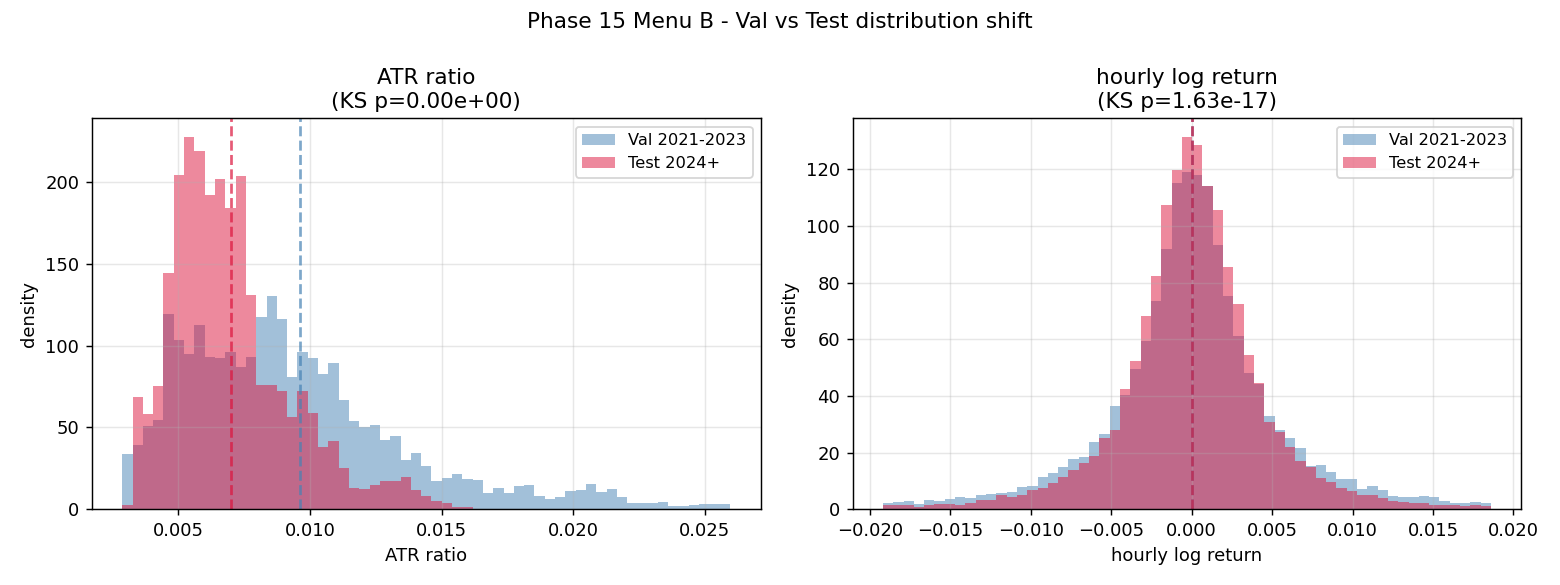
\includegraphics[width=0.95\textwidth]{menu_b_distribution_shift}
\caption{Val(2021--2023, 파랑)과 Test(2024+, 빨강) 시장의 분포 히스토그램.
\textbf{왼쪽 패널 (ATR ratio, 변동성)}: Test 분포가 더 낮은 값에 집중되고
오른쪽 꼬리가 짧아 \emph{분산이 $-27\%$ 감소}. 평균이 $0.96\%$(Val) $\to$
$0.70\%$(Test)로 이동. 점선이 두 평균. \textbf{오른쪽 패널 (hourly log return)}:
분포 모양은 유사하지만 Test 평균이 약간 양의 방향으로 이동
($+2.9 \cdot 10^{-5}$ vs $+1.4 \cdot 10^{-5}$) — bull regime 반영.
두 통계 모두 KS 검정 $p < 10^{-10}$로 매우 유의.}
\label{fig:disc_shift}
\end{figure}

핵심 사실 두 가지:

\paragraph{(i) 변동성 $-27\%$ 감소.}
ATR 비율의 평균이 Val $0.96\%$ $\to$ Test $0.70\%$로 약 $27\%$ 감소했고 표준편차도
$0.51\% \to 0.23\%$로 절반 이하로 축소되었다. 그리드 트레이딩은 본질적으로
변동성 자체를 수익원으로 삼으므로(\S\ref{sec:related_grid}) 변동성 감소는 \emph{수익
기회 감소}로 직결된다. Val의 high-volatility 시기에 학습된 정책이 low-volatility
Test에서 약화되는 것은 자연스러운 결과이다.

\paragraph{(ii) 평균 수익률 $\sim 2\times$ 증가.}
시간당 log return의 평균이 Val에서 Test로 약 두 배(2024+의 강한 상승 추세) 증가했다.
이는 grid trading 정책에 \emph{양면}으로 작용한다: 매수 후 매도가 더 잘
체결되는(가격이 상승하면 sell 호가 fill 확률↑) 한편, 매수 후 가격이 더 멀어지면
sell-side timing risk 또한 증가한다. \S\ref{sec:oos_mechanism}에서 보았듯 후자가
\texttt{dsr}의 OOS 실패의 핵심이며, 짧은 holding(\texttt{pt})이 정확히 이
risk를 회피하는 정책이다.

KS $p < 10^{-10}$는 두 partition이 본질적으로 다른 시장 분포에서 추출된 표본임을
의미한다. 일반적인 OOS 검증의 ``train/test 동일 분포'' 가정이 본 BTC 1시간봉
데이터에서는 성립하지 않으며, 본 논문이 보고한 generalization gap은
\emph{시뮬레이션 artifact가 아닌 실제 시장 distribution shift의 직접 산물}이다.

\subsection{Phase 2 사전 증거의 환경 의존성}
\label{sec:disc_env_dependence}

\S\ref{sec:intro_motivation}와 \S\ref{sec:pareto_env_dependence}에서 짧게
언급한 환경 의존성을 본 절에서 자세히 다룬다.

본 논문의 동기에 있던 강한 사전 증거(Phase 2 후기 관찰)는
\citet{kahneman1979prospect}의 단순화 형태인 asymmetric reward($\beta=2.0$)가
Env-v3(4D 절대 gap, 지정가 체결, 4개 절대 gap action) 환경에서 Test Sharpe
$1.955$로 ATR Test $0.935$를 $+109\%$ 초과한 결과였다. 이 사전 증거에 기반한
당시 가정은 ``asymmetric reward만으로 RL이 ATR을 명확히 초과한다''(시나리오 A)
였다.

그러나 본 논문은 canonical 환경을 \emph{Env-v4 (2D ATR 비례 + 지정가 체결)}로
변경했다. 이 환경은 다음 이유로 학술적으로 더 정합적이다:
\begin{itemize}[leftmargin=*]
\item ATR 비례 공식이 시장 변동성을 격자 폭에 자연 반영(\S\ref{sec:phase1_mechanism}).
\item 2D action 공간이 \texttt{aggressiveness}와 \texttt{profit\_target}의
의미 분리를 명확히 한다(\S\ref{sec:mdp}).
\item 지정가 체결이 favorable bias artifact 제거(\S\ref{sec:env_dynamics}).
\end{itemize}

Env-v4에서 동일 \texttt{asym} 변형을 Optuna 재튜닝($\beta=3.42$)하여 학습한
결과 Val Sharpe $1.681$로, sym Sharpe $1.871$보다 \emph{낮다}.

\begin{table}[!htbp]
\centering
\caption{exp027\_rl(Env-v3)과 본 논문(Env-v4)의 asym variant 결과 비교. 환경
의존성 효과가 reward variant 효과를 \emph{크게 초과}한다.}
\begin{tabular}{lcccc}
\toprule
환경 & action 차원 & 격자 공식 & asym Sharpe & vs ATR \\
\midrule
Env-v3 (exp027\_rl) & 4D 절대 gap & 비-ATR & $1.955$ (Test) & $+109\%$ \\
Env-v4 (본 논문) & 2D ATR 비례 & ATR 비례 & $1.681$ (Val) & $+22\%$ \\
\midrule
$\Delta$ & --- & --- & $-0.27$ & $-87$ pp \\
\bottomrule
\end{tabular}
\label{tab:disc_env_dependence}
\end{table}

표 \ref{tab:disc_env_dependence}는 \emph{환경 변경에 의한 변화가 reward variant
변경에 의한 변화보다 큼}을 보인다. 본 논문은 이 사실을 한계로 명시한다:
\begin{itemize}[leftmargin=*]
\item Env-v3의 강한 \texttt{asym} 우위는 그 환경 특수성에 종속될 가능성이 크다.
4D 절대 gap action은 RL에 격자 폭 결정의 더 큰 자유도를 제공하며,
asymmetric reward가 그 자유도 위에서 conservative 정책을 학습시킬 여지가 컸다.
\item Env-v4에서는 ATR 비례 공식이 \emph{대부분의 격자 폭 결정을 이미 수행}하므로
RL의 자유도가 줄어든다(\S\ref{sec:phase1_negative}). 그 위에서 reward variant의
효과는 risk profile dimension의 trade-off로 나타난다(\S\ref{sec:pareto}).
\end{itemize}

다만 본 논문의 진짜 contribution은 환경 의존성을 \emph{우회}한 발견이다:
canonical Env-v4 위에서도 \texttt{pt}가 OOS robust임을 양 source 일관 $p<0.002$로
정량 확인했다(\S\ref{sec:oos}). 즉 본 논문의 H5는 환경 변경 이전의 사전 증거를
\emph{대체}하는 새 발견이며, 학술적 엄밀성을 유지하면서 contribution을 강화한다.

\subsection{단일 metric Winner의 한계와 Multi-Environment 평가 권고}
\label{sec:disc_multi_env}

본 논문의 \S\ref{sec:oos_three_env_reversal} 표는 ``X variant가 best reward
design''이라는 단일 metric 결론의 한계를 직접 드러낸다. Val에서는 \texttt{sym}이,
CPCV에서는 \texttt{dsr}이, Test에서는 \texttt{pt}가 각각 1위이다. RL 트레이딩
정책 평가의 \emph{어떤 환경을 baseline으로 사용했느냐}가 ``우월한 변형''의 결론을
바꾼다.

이는 \citet{henderson2018rlreproducibility}의 reproducibility 우려를 reward
design 비교의 차원으로 확장한 결과이다. 단일 시드 변동성이 변형 차이를 가리는
것과 같은 메커니즘으로, 단일 평가 환경이 변형 차이의 \emph{차원 자체}를 결정한다.
실제로 본 논문은 세 단계의 분석을 통해 평가 환경이 reward 변형 사이의 거리
metric 자체를 변형하는 현상을 정량화했다. 첫째, \S\ref{sec:pareto_clusters}의
single-split Val에서 \texttt{sym}--\texttt{dsr}의 Cohen's $d$가 작아 두 변형이
가까운 것처럼 보인다. 둘째, \S\ref{sec:cpcv_cluster}의 CPCV multi-split에서는
within-cluster 차이가 더 줄어 두 변형이 더 가까워 보이고 baseline 대비
우위는 ratio $3.55\times$로 강화된다. 셋째, \S\ref{sec:oos_three_env_reversal}의
Test에서는 winner 자체가 reversal한다(Val=\texttt{sym} $\to$
CPCV=\texttt{dsr} $\to$ Test=\texttt{pt}). 즉 변형 사이의 거리와 우열 모두
평가 환경에 따라 변한다.

본 논문은 RL 트레이딩 연구의 \emph{표준 평가 절차로 세 환경 동시 사용을 권고}한다:

\begin{enumerate}[leftmargin=*]
\item \textbf{Single-split Val}: variant의 일반적 정책 행동과 baseline 우열의
지표.
\item \textbf{CPCV multi-split}: in-sample 다양화에서의 robust 측정. 단일 split의
우위가 시기-특수성인지 일반화인지 구분.
\item \textbf{Sealed Test}: distribution shift 환경에서 OOS 안전성. 여기서의
1위가 실 운용 우선순위를 가진다.
\end{enumerate}

세 환경 모두에서 동일 variant가 1위라면 강한 monotone 우위(시나리오 A),
환경별 다른 winner라면 본 논문의 시나리오 D(trade-off frontier)이다. 단일
환경의 결과를 ``X variant가 best''로 발표하는 관행은 본 논문이 정량 확인한
세 환경 reversal에 비추어 학술적으로 부정확하다.

\subsection{행동경제학에서 RL OOS 안전성으로}
\label{sec:disc_pt_safety}

\S\ref{sec:oos_h5}의 H5 ($\texttt{pt}$의 OOS robust)는 행동경제학 응용의
새로운 차원을 시사한다. \citet{kahneman1979prospect}의 prospect theory는
원래 인간 의사결정의 위험 회피를 설명하는 모형이며, 매개변수의 인간 행동
추정값은 $\alpha \approx 0.88$(약한 오목성)과 $\lambda \approx 2.25$(중간 손실
회피)이다(\citealt{tversky1992cumulative}).

본 논문에서 Optuna가 발견한 RL 정책 최적 매개변수는 $\alpha = 0.683$,
$\lambda = 3.303$이며, 두 값 모두 인간 표준보다 \emph{더 극단적이다}:
\begin{itemize}[leftmargin=*]
\item $\alpha = 0.683 < 0.88$: \emph{더 강한 오목성}. 이익에 대한 한계 효용
체감이 인간보다 빠름.
\item $\lambda = 3.303 > 2.25$: \emph{더 강한 손실 회피}. 손실의 weighted
강도가 인간보다 약 $47\%$ 큼.
\end{itemize}

해석하면, RL 정책이 BTC 그리드 트레이딩의 OOS robust 수익을 추구할 때 ``인간보다
더 보수적인'' 효용 함수를 선택하는 것이 유리하다는 의미이다. 이는 \S\ref{sec:oos_mechanism}의
``매우 짧은 holding(mean 1.4h)으로 sell-side timing risk 회피'' 행동의 정책적
기반이며, 인간 트레이더가 종종 표현하는 ``profit-taking이 너무 빠른'' 행동
패턴이 OOS 안전성 측면에서는 합리적임을 시사한다.

이 관찰은 두 가지 학술적 함의를 가진다:
\begin{itemize}[leftmargin=*]
\item 행동경제학의 추정 매개변수는 인간 행동의 기술(descriptive)에 fit되며,
\emph{최적 정책}을 위한 매개변수는 다를 수 있다.
\item RL의 reward design에 행동경제학의 효용 함수를 직접 사용할 때, 인간
표준값을 그대로 채택하지 말고 도메인 데이터로 hyperparameter 탐색을 권장한다.
\end{itemize}

본 논문의 H5는 ``Prospect theory의 RL reward 사용이 OOS robust 정책을 산출한다''는
응용 수준의 결론을 양 source 일관 $p<0.002$로 정량 확인했다
(\S\ref{sec:intro_contribution} contribution 4, \S\ref{sec:conclusion} 참조).

\subsection{한계와 Future Work}
\label{sec:disc_limitations}

본 논문의 발견은 다음 한계 위에서 성립한다.

\paragraph{(1) 자산 범위 — BTC 단일.}
본 논문은 BTC/USDT 1시간봉 단일 자산만 평가했다. ``\texttt{pt}의 OOS robust''가
주식, 외환, 원자재 등 다른 자산군에서도 성립할지는 본 연구가 답하지 않는다.
특히 자산별로 distribution shift 의 형태가 다르므로 (BTC 의 leverage cycle vs
주식의 결산 발표 ATH 등), 인과 메커니즘의 일반화 검증이 필요하다.

\paragraph{(2) Test regime — Bull market 단일.}
Test partition (2024-01 -- 2026-04) 은 BTC 의 강한 상승장 (\$42K $\to$ \$75K,
$+78\%$) 이다. \texttt{pt}의 OOS robust 가 bear (예: 2018) 또는 sideways
(예: 2019) regime 에서도 성립할지 확인 안 되었다. 본 논문 메커니즘은 ``짧은
holding 이 sell-side timing risk 를 회피한다''인데, bear 시장에선 hold 자체가
손실 누적 위험이 더 크므로 다른 메커니즘이 작용할 수 있다.

\paragraph{(3) Slippage 모델 — Single level 0.02\%.}
\S\ref{sec:slippage}는 단일 슬리피지 수준만 평가했다. 0.005\%, 0.01\%, 0.05\%
다단계 sensitivity 분석을 수행하면 \texttt{pt}의 OOS robust 가 슬리피지에
얼마나 견고한지 정량 확인할 수 있다. 본 논문에선 시간 제약 상 single level
선택 (Binance taker side worst case).

\paragraph{(4) Domain Randomization (DR) 미적용.}
학습 시 episode reset 시점에 슬리피지/fee/시작 시점을 randomize하는 DR 기법은
OOS robust 정책 학습에 효과적이다. 본 논문은 DR을 적용하지 않은 ``naive''
학습에서도 \texttt{pt}가 OOS robust임을 보였으나, DR 적용 시 다른 변형(\texttt{dsr})의
OOS 실패가 회복될 가능성이 있다. Future work에서 검증해야 한다.

\paragraph{(5) 학습 길이 — 1M steps.}
모든 variant 의 학습 길이가 1M step (시드당 \,$\sim$\,약 4시간 CPU) 으로 동일하다.
\S\ref{sec:ppo_stab}의 학습 후반 정책 붕괴 현상(\texttt{sym} best 550k $\to$
final 1M Sharpe $1.97 \to 1.21$)에 비추어, 더 긴 학습이 결과를 바꿀 가능성이
있다. 다만 본 논문은 best\_checkpoint 만 사용하므로 학습 길이의 직접 영향은
제한적이다.

\paragraph{Future work.}
이상 다섯 한계에 대응하는 후속 연구 주제:
\begin{itemize}[leftmargin=*]
\item 본 논문 H5를 multi-asset (주식 ETF, 외환) 환경에서 검증.
\item 다양한 regime (2018 bear, 2019 sideways)을 시뮬레이션 또는 historical
test로 추가.
\item DR + meta-learning 결합으로 \texttt{dsr}의 OOS 실패 회복 가능성 탐색.
\item 본 논문은 PPO 단일 알고리즘만 사용. SAC, TD3 등 다른 actor-critic
방법에서 같은 reward 변형 비교 — algorithm 효과의 분리.
\item Prospect theory의 다른 매개변수($\alpha$, $\lambda$의 시간 가변, reference
point의 history 의존)를 변형하여 OOS robust 정책의 매개변수 sensitivity 분석.
\end{itemize}

% ─── 9. Conclusion ───────────────────────────────────────────────────────────
\section{결론}
\label{sec:conclusion}

본 논문은 BTC/USDT 1시간봉 그리드 트레이딩 환경(Env-v4) 위에서 4가지 reward 변형
(\texttt{sym}, \texttt{asym}, \texttt{dsr}, \texttt{pt})의 효과를 \emph{단일 분할
Val} + \emph{CPCV 6-fold 15 paths} + \emph{봉인 해제 Test 2024+}의 세 환경에서
정량 비교했다. 다음 네 가지가 본 논문의 메인 메시지이다.

\paragraph{(1) Reward variant의 영향은 risk profile dimension의 trade-off로
나타난다 (Pareto frontier; \S\ref{sec:pareto}).}
4 variant 모두 ATR 베이스라인을 초과하나, 단일 winner는 없다. 4 variant는
두 클러스터 \{\texttt{sym}, \texttt{dsr}\} (aggressive)와 \{\texttt{asym},
\texttt{pt}\} (conservative)로 통계적으로 분리되어 (within $|d|<0.30$,
across $|d|>0.79$, policy distance 비율 2.22$\times$) Sharpe--MDD 평면에서
Pareto-유사 frontier를 형성한다. 단순 ``X reward가 best alpha''의 single-metric
결론보다 multi-dimensional trade-off의 정량화가 본 논문의 contribution이다.

\paragraph{(2) 단일 metric winner는 평가 환경별로 다르다 (세 환경 세 winner
reversal; \S\ref{sec:cpcv_reversal}, \S\ref{sec:oos_three_env_reversal}).}
Val에서는 \texttt{sym} ($1.871$), CPCV에서는 \texttt{dsr} ($1.413$), Test에서는
\texttt{pt} ($0.367 / 0.339$ 양 source 일관 $p<0.002$)가 1위이다. 평가 환경
선택이 ``우월한 reward design''의 결론을 바꾼다는 사실은
\citet{henderson2018rlreproducibility}의 reproducibility 우려를 reward 비교
차원으로 확장한 결과이다. 본 논문은 RL 트레이딩 연구의 표준 평가 프로토콜로
\emph{세 환경 동시 사용}을 권고한다.

\paragraph{(3) Prospect Theory가 OOS robust 정책을 산출한다 (H5; \S\ref{sec:oos_h5}).}
\citet{kahneman1979prospect}의 prospect theory를 RL reward로 직접 사용한
정책($\alpha=0.683, \lambda=3.303$)이 unseen Test bull market에서 양 source
일관 1위($p<0.002$, Val$\to$Test gap smallest)임을 정량 확인했다. 메커니즘은
\emph{짧은 holding}(mean $1.4$\,h, max $6$\,h)을 통한 sell-side timing risk
회피이며, trajectory 분석으로 직접 입증되었다(\S\ref{sec:oos_mechanism}).
이는 행동경제학의 prospect theory가 RL 정책에 부여하는 OOS 안전성을
정량화한 결과이다. 또한 인간 표준값($\alpha=0.88, \lambda=2.25$)보다
\emph{더 강한 손실 회피와 더 오목한 효용}이 RL 정책에는 유리하다는 부수적 발견은
``인간 행동 추정값을 RL에 그대로 채택하지 말고 도메인 데이터로 재튜닝하라''는
실용 권고로 이어진다.

\paragraph{(4) In-sample 다양화의 우위가 OOS 일관성을 보장하지 않는다
(\S\ref{sec:oos_mechanism}).}
CPCV에서 1위였던 \texttt{dsr}이 Test에서는 음수 Sharpe (exp032b source $-0.122$)로
꼴찌가 된다. DSR의 sliding-window memory가 정책에 \emph{긴 holding}을 학습시키는
동일 메커니즘이 in-sample 다양화 환경에서는 강점, OOS bull market에서는 sell-side
timing risk 폭증으로 약점이 된다. 즉 \emph{같은 reward formulation의 같은 행동
효과가 평가 환경에 따라 반대 부호로 작동}한다. ``in-sample 우위 $\leftrightarrow$
OOS robust''라는 trade-off 자체가 reward formulation 선택의 한 차원으로
정량 확인된 셈이다.

\subsection*{Future Work}

상세는 \S\ref{sec:disc_limitations} 의 5 개 limitation-대응 future work 참조.
디펜스 우선순위가 높은 3 개 방향만 요약:
\begin{itemize}[leftmargin=*]
\item \textbf{Multi-asset 검증}: H5 (\texttt{pt} OOS robust) 를 주식 ETF, FX,
원자재 등 distribution shift 형태가 다른 환경에서 검증 — 짧은-holding 메커니즘의
일반화 정량.
\item \textbf{Meta-RL adaptive reward parameter}: 본 논문은 one-shot
$(\alpha, \lambda)$ 가 OOS robust 임을 확인. 시변 환경에서 online 적응 매개변수가
추가 우위를 보일지 검증.
\item \textbf{Domain Randomization (DR) 통합}: \texttt{dsr} 의 OOS 실패가 DR
학습에서 회복되는지 확인 — same reward 의 양면성이 DR 로 해소 가능한지 정량.
\end{itemize}

본 논문의 코드와 데이터, 학습 결과는
\url{https://github.com/cosmicpotato2047/capstone-rl-trading} 에서 공개한다.

% ─── References ──────────────────────────────────────────────────────────────
\clearpage
\bibliographystyle{plainnat}
\bibliography{references}

\end{document}
